\documentclass[12pt,a4paper]{article}
\usepackage{blindtext}\usepackage{accsupp}

\usepackage{amssymb}
\usepackage{wasysym}
\usepackage{mathrsfs}
\usepackage[utf8]{inputenc}
\usepackage{physics} % Assuming you resolved the package conflicts
\usepackage{anyfontsize}
\usepackage{amsmath,mathtools}
\usepackage{amssymb}
\usepackage{mathrsfs}
\usepackage[margin=0.65in]{geometry}
\usepackage{xcolor}
\usepackage{fancyhdr}
\usepackage{amsfonts}
\usepackage[euler]{textgreek}
\usepackage{chemformula}
\usepackage{titlesec} % For customizing section heading sizes
\usepackage{indentfirst} % For indenting the first paragraph of each section
\usepackage[hidelinks]{hyperref} 
\usepackage{tabularx}
\usepackage{graphicx}
\usepackage{array}
\usepackage{listings}
\usepackage{xcolor}
\usepackage{pdfpages}
\usepackage{booktabs}
\usepackage{enumitem}
% Custom headers and footers using fancyhdr package
\pagestyle{fancy}
\fancyhead[L]{\footnotesize INP-UGA ENES3 M2 SGB}
\fancyhead[R]{\footnotesize New Sustainable Technoglogies}
\fancyhead[C]{\footnotesize 2024 - 2025}
\renewcommand{\headrulewidth}{0.5pt}
\renewcommand{\footrulewidth}{0.5pt}
\fancyfoot[R]{\textcolor{black}{\footnotesize SARY MONYCHOT \& NIANG BORA}}
\fancyfoot[L]{\footnotesize}

% Set up table formatting
\setlength{\arrayrulewidth}{0.5mm}
\setlength{\tabcolsep}{15pt}
\renewcommand{\arraystretch}{0.95}

% Custom command for electron representation

\newcolumntype{C}{>{\centering\arraybackslash}X}
% Customize section heading sizes
\titleformat{\section}{\normalfont\large\Roman{\bfseries}}{\thesection}{1em}{}
\titleformat{\subsection}{\normalfont\normalsize\bfseries}{\thesubsection}{0.75em}{}
\titleformat{\subsubsection}{\normalfont\normalsize\bfseries}{\thesubsubsection}{0.5em}{}

% Customize equation numbering to include section number
\numberwithin{equation}{section}
\lstset{ 
	language=Python,                 % the language of the code
	basicstyle=\ttfamily\footnotesize, % the size of the fonts that are used for the code
	numbers=left,                   % where to put the line-numbers
	numberstyle=\tiny\color{gray},  % the style that is used for the line-numbers
	stepnumber=1,                   % the step between two line-numbers. If it's 1, each line will be numbered
	numbersep=5pt,                  % how far the line-numbers are from the code
	backgroundcolor=\color{white},      % choose the background color. You must add \usepackage{color}
	showspaces=false,               % show spaces adding particular underscores
	showstringspaces=false,         % underline spaces within strings
	showtabs=false,                 % show tabs within strings adding particular underscores
	frame=single,                   % adds a frame around the code
	rulecolor=\color{black},        % if not set, the frame-color may be changed on line-breaks within not-black text (e.g. comments (green here))
	tabsize=4,                      % sets default tabsize to 2 spaces
	captionpos=b,                   % sets the caption-position to bottom
	breaklines=true,                % sets automatic line breaking
	breakatwhitespace=false,        % sets if automatic breaks should only happen at whitespace
	keywordstyle=\color{blue},      % keyword style
	commentstyle=\color{green},   % comment style
	stringstyle=\color{red},      % string literal style
}

\begin{document}
	\title{\textbf{PEM Fuel Cell system analysis }}
	\author{SARY Monychot \& NIANG Bora }
	%\date{\today}
	\maketitle
		% Table of Contents
	\tableofcontents
% =============================================================	
		\newpage
%% =======================================1 . =========================================
	% Sections and Subsections
	\section{\underline{Calculation of the power demand inside the vechicle}}
	\begin{itemize}
	 \item The specification of the vehicle are the following:
	
	\begin{itemize}
		\item  Weight $M = 2000 kg$
		\item Front area $A = 2.25  m^2$
		\item Drag coefficient (or air penetration coefficient) $C = 0.29$ 
		\item Rolling Resistance coefficient $C_r = 0.0115$
		
	\end{itemize}
	
	\item The efforts applied on the vehicle in the rolling direction have to following expression:
	
	\begin{itemize}
		\item Air penetration : 
		\begin{equation}
				F{(t)} = \frac{1}{2}\rho_{air}v^2_{(t)}CA  \label{eq1}
		\end{equation} with $\rho_{air} = 1.2    kg/m^3$
		\item Rolling resistance :	
		\begin{equation}
			 F(t) = MgC_r\cos{\alpha} \label{eq2}
		\end{equation}with $g = 9.81 m/s^2$ and $\alpha$ the slope angle
		\item Climbing or descent : 
		\begin{equation}
			F(t) = Mg\sin{\alpha} \label{eq3}
		\end{equation} 
		
	\end{itemize}
	\end{itemize}
	
	
%% ======================================= a . =========================================	

	\subsection{Calculate and plot the instant power provided by the vechicle powertrain for the road cycles " WLTC " }
	
	$\star$ Consider a flat road $(\alpha = 0)$
	\begin{figure}[htbp]
		\centering
		\begin{tabular}{c @{\qquad} c}
			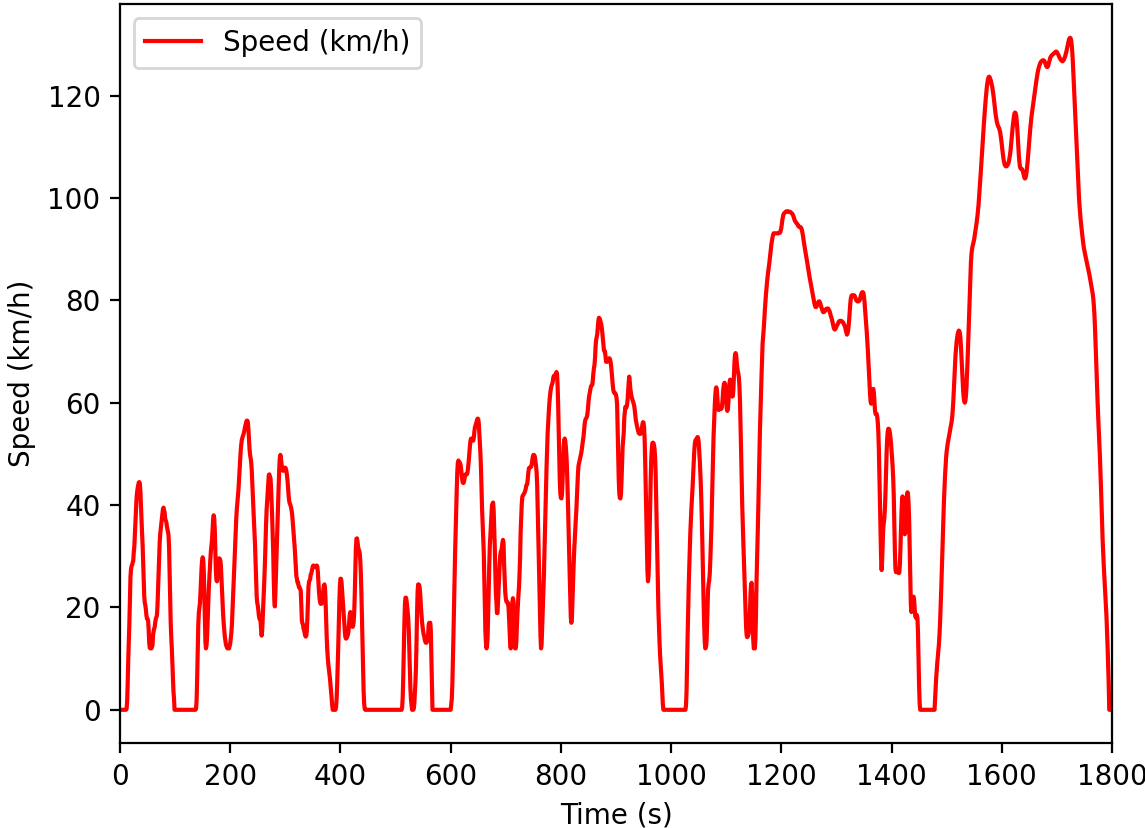
\includegraphics[width=0.48\linewidth]{E:/07. Master_Degree_ITC+UGA/02. ENES3_SGB_UGA/02. New Technology/PEMFC/Speed_1.png} &
			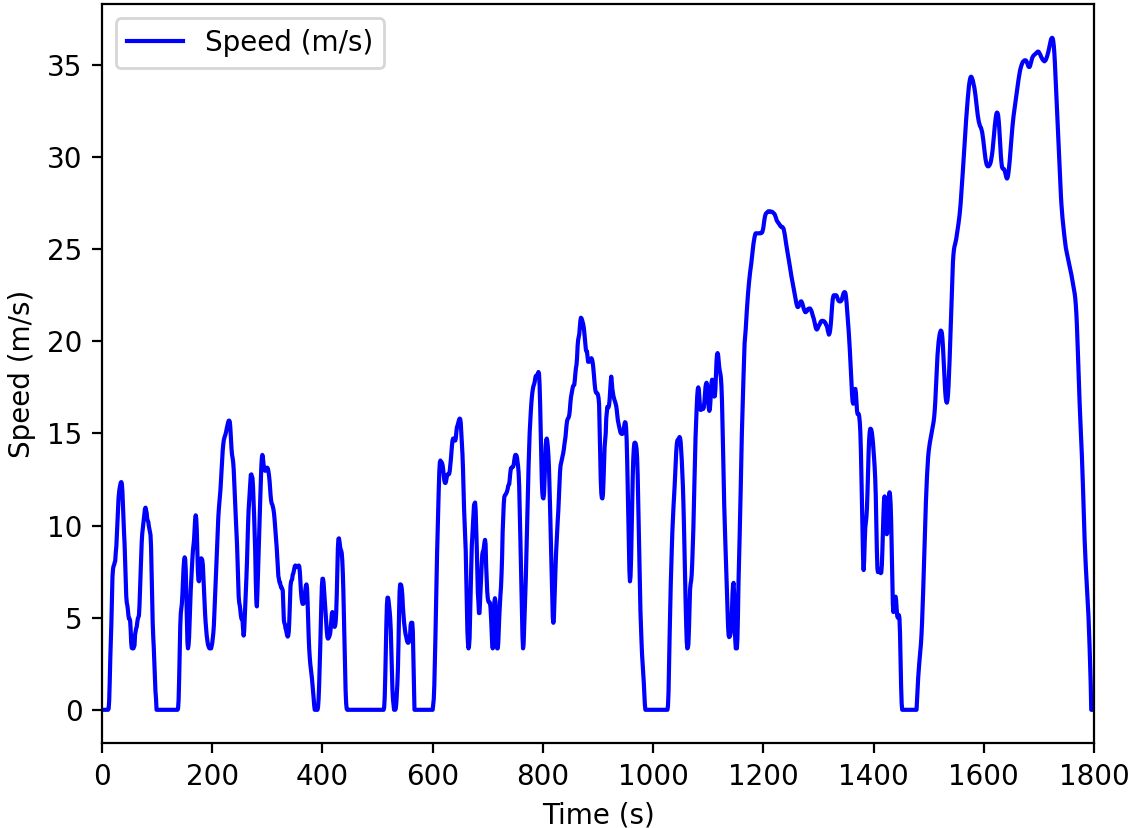
\includegraphics[width=0.48\linewidth]{E:/07. Master_Degree_ITC+UGA/02. ENES3_SGB_UGA/02. New Technology/PEMFC/Speed ms-1_1.png} \\
			
			\small (a) Speed Profile in km/h & \small (b) Speed Profile in m/s
		\end{tabular}
		
		\caption{\small Graph of the Speed Profile in km/h and Speed in m/s}
		\label{1}
	\end{figure}

%% ========================================================================================================
	\subsubsection{Calculation}
	
	To calculate the \textbf{Instant Power}, we need to study of the \textit{force} that have action on the car. By using second Newton's law with the Figure (\ref{2}) shown below, we can assume that there are 4 forces that have action on thecar while driving.
	
	\begin{figure}[h]
		\centering 
		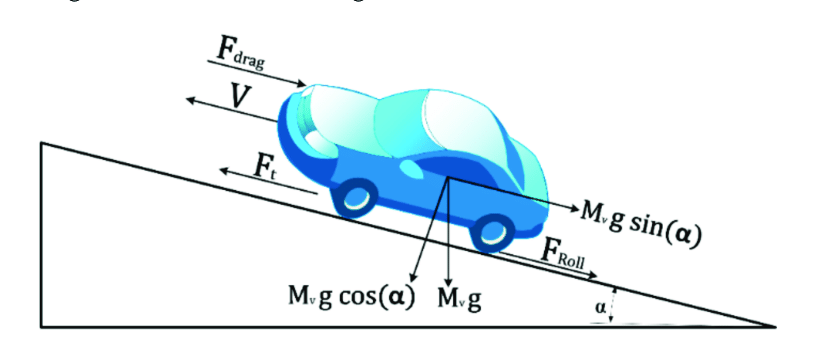
\includegraphics[width=0.7\linewidth]{E:/07. Master_Degree_ITC+UGA/02. ENES3_SGB_UGA/02. New Technology/PEMFC/2.png}
		\caption{\small {Speed (km/h) of the vechicle powertrain by time (s)}}
		\label{2}
	\end{figure}



	\begin{itemize}
		\item The first force is to make the car move in direction. It called the force from motor or machine of the car ($F_{motor}$)
		\item The second force is the rolling force from the car wheels. It called \textbf{Rolling Resistance} ($F_{rolling}$)
		\item The third force is the climbing or descent force ($F_{climb}$)
		\item The fourth force is the force from the air friction. we can called it Air penetration ($F_{air}$).
	\end{itemize}


	Using second Newton's law, we can written :
	\begin{equation}
		\overrightarrow{F}_{motor} - \overrightarrow{F}_{rolling} -\overrightarrow{F}_{climb} - \overrightarrow{F}_{air} = m\overrightarrow{a}
		\label{eq4}
	\end{equation}
	\begin{equation}
		\overrightarrow{F}_{motor} = \overrightarrow{F}_{rolling} + \overrightarrow{F}_{climb} + \overrightarrow{F}_{air} + m\overrightarrow{a}
		\label{eq5}
	\end{equation}

	since $a$ is the acceleration of the vechical in time $t$, as we written : 
	\begin{equation}
		\overrightarrow{a} = \derivative{\overrightarrow{v}}{t} = \frac{\Delta v}{\Delta t}
		\label{eq6}
	\end{equation}

	By using Equation (\ref{eq6}), we can get the result of acceleration on the Figure (\ref{3})
	\begin{figure}[h]
		\centering 
		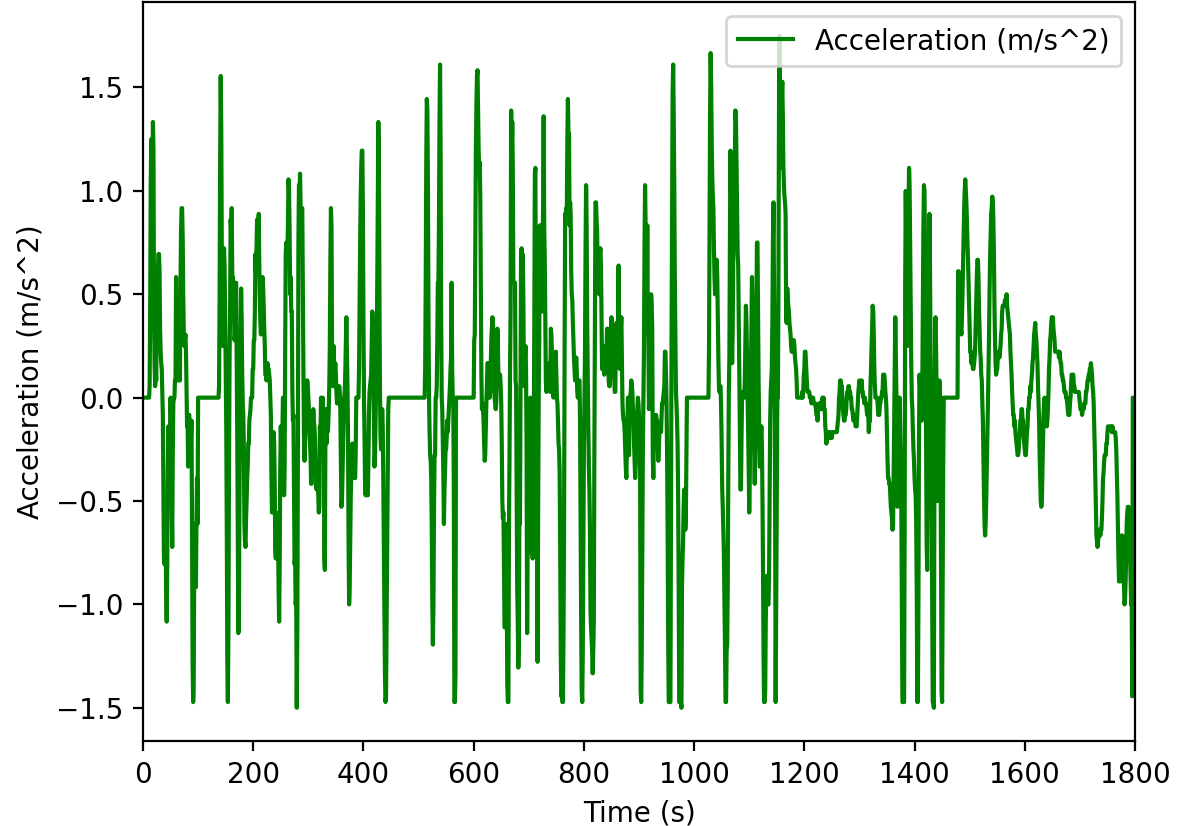
\includegraphics[width=0.65\linewidth]{E:/07. Master_Degree_ITC+UGA/02. ENES3_SGB_UGA/02. New Technology/PEMFC/Acceleration_1.png}
		\caption{\small {Acceleration $(m/s^2)$ of the vechicle powertrain by time (s)}}
		\label{3}
	\end{figure}

	According to the graph, it shown that the vechical did not have the stable speed drive on the. At the some time ($t$), the vechical increasing the speed immediately. In contrast, at some time ($t$), the vechical reducing the speed quickly as shown in the Figure (\ref{3}).

	\begin{itemize}[label=-]
		\item For calculate $F_{air}$ by using Equation (\ref{eq1}) , we got :
			\begin{equation}




				F_{air}(t) = \frac{1}{2}\rho_{air}v^2CA = \frac{1}{2}\times1.2\times 	v^2_{m/s}_{,t}\times0.29\times 		2.25 \label{eq7}
			\end{equation}
			In this section, to calculate $F_{air}$ we need to get the speed in each time $t$ in $m/s^2$ to analyze in the Equation (\ref{eq7})
			By using the Equation (\ref{eq1}), we got the result of the force air penetration by shown in below graph.
		\item For calculate $F_{rolling}$, we will be using the Equation (\ref{eq2}), we got :
			\begin{equation}
				F_{rolling}(t) = MgC_r\cos(\alpha) = 2000kg\times9.81m/s^2\times0.0115\times\cos(0^\circ) = \textbf{225.630} \label{eq8}
			\end{equation}
			For this force, it will be constant in time $(t)$ becuase there is not any parameter in the Equation (\ref{eq8}) will change in which time.
			
			
		\item For calculate $F_{climb}$, we will use Equation (\ref{eq4}) then we got:
		
			\begin{equation}
				F_{climb}(t) = Mg\sin(\alpha) = 2000kg \times 9.81m/s^2 \times \sin(0^\circ) = 0 \label{eq9}
			\end{equation}		
	\end{itemize}

	By using Equation (\ref{eq6}), (\ref{eq7}), (\ref{eq8}) and (\ref{eq9}) substitution into Equation (\ref{eq5}). The result of total force was shown by the graph in Figure (\ref{4}).
	
	\begin{figure}[htbp]
		\centering
		\begin{tabular}{c @{\qquad} c}
			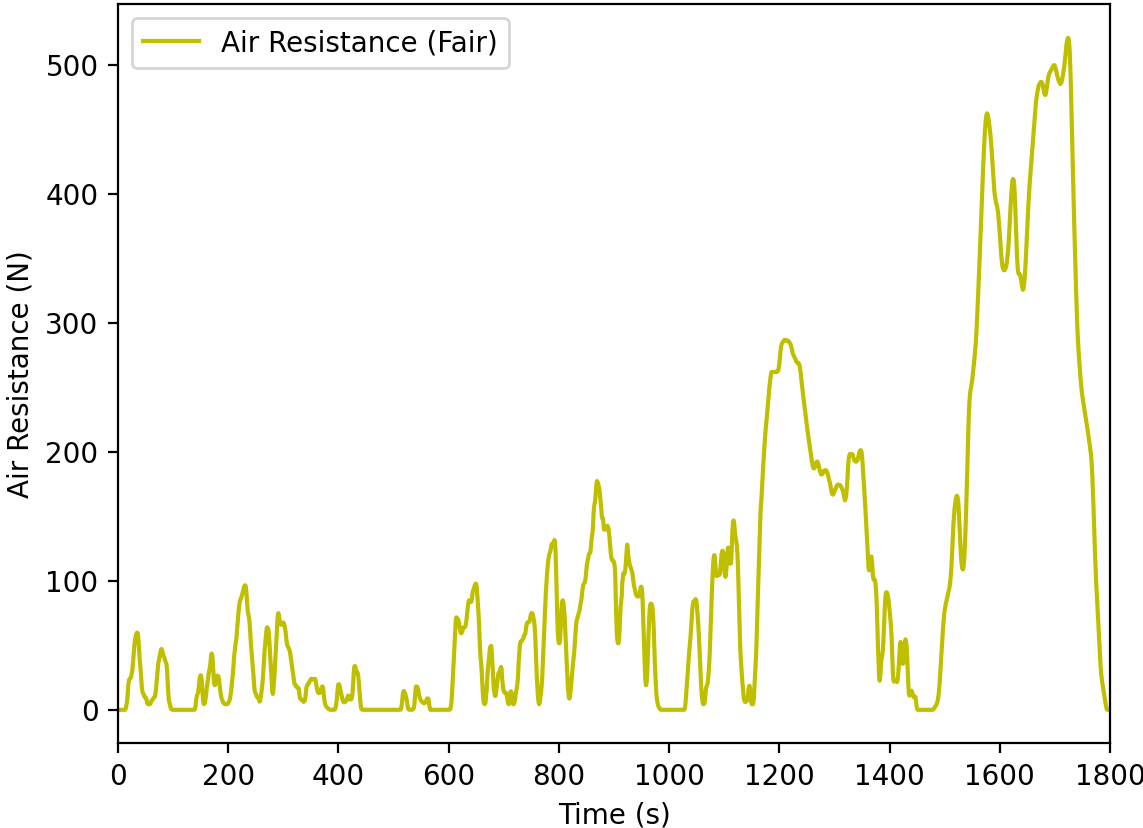
\includegraphics[width=0.48\linewidth]{E:/07. Master_Degree_ITC+UGA/02. ENES3_SGB_UGA/02. New Technology/PEMFC/Fair_1.png} &
			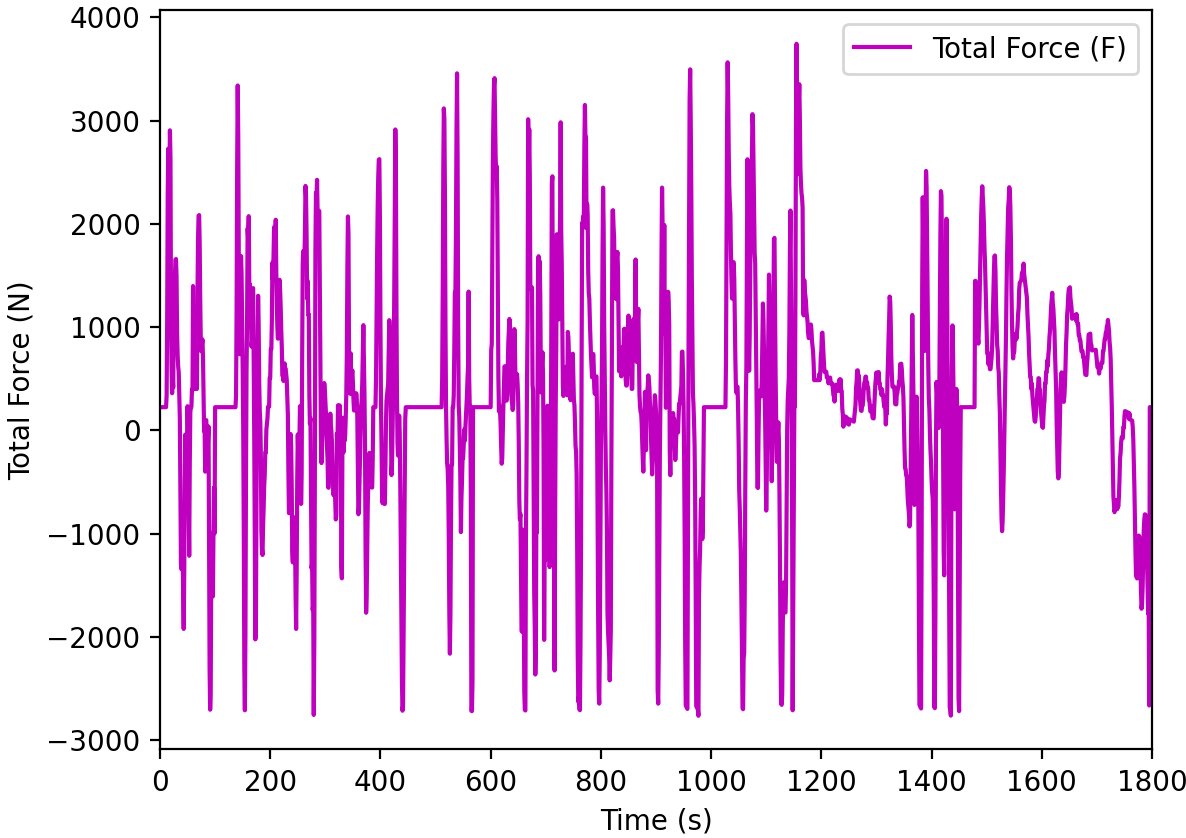
\includegraphics[width=0.48\linewidth]{E:/07. Master_Degree_ITC+UGA/02. ENES3_SGB_UGA/02. New Technology/PEMFC/Total_Force_1.png} \\
			
			\small (a) Force of Air Resistance & \small (b) Total Force
		\end{tabular}
		
		\caption{\small Graph of the  Force of Air Resistance and Total Force}
		\label{4}
	\end{figure}
		
	To calculate Instant power we are using :
	
	\begin{equation}
		P = F \times v \label{eq10}
	\end{equation}	
	
	The result of the instant power calcuation will be show at Figure (\ref{5})b. The instant power of the vechical are depend on two parameter :
	\begin{itemize}
		\item The total force from the vechical action ($N$).
		\item The speed that make the vechical go forward ($m/s$).
	\end{itemize}	                                                                                                                                                                  
	\indent As now, we can write that 
		\begin{equation}
			P_t = F_t \times v_t 
		\end{equation} 
	\newpage
	
	 The result of the instant power will show in the Figure ({\ref{5}).
	 
	 \begin{figure}[h]
	 	\centering 
	 	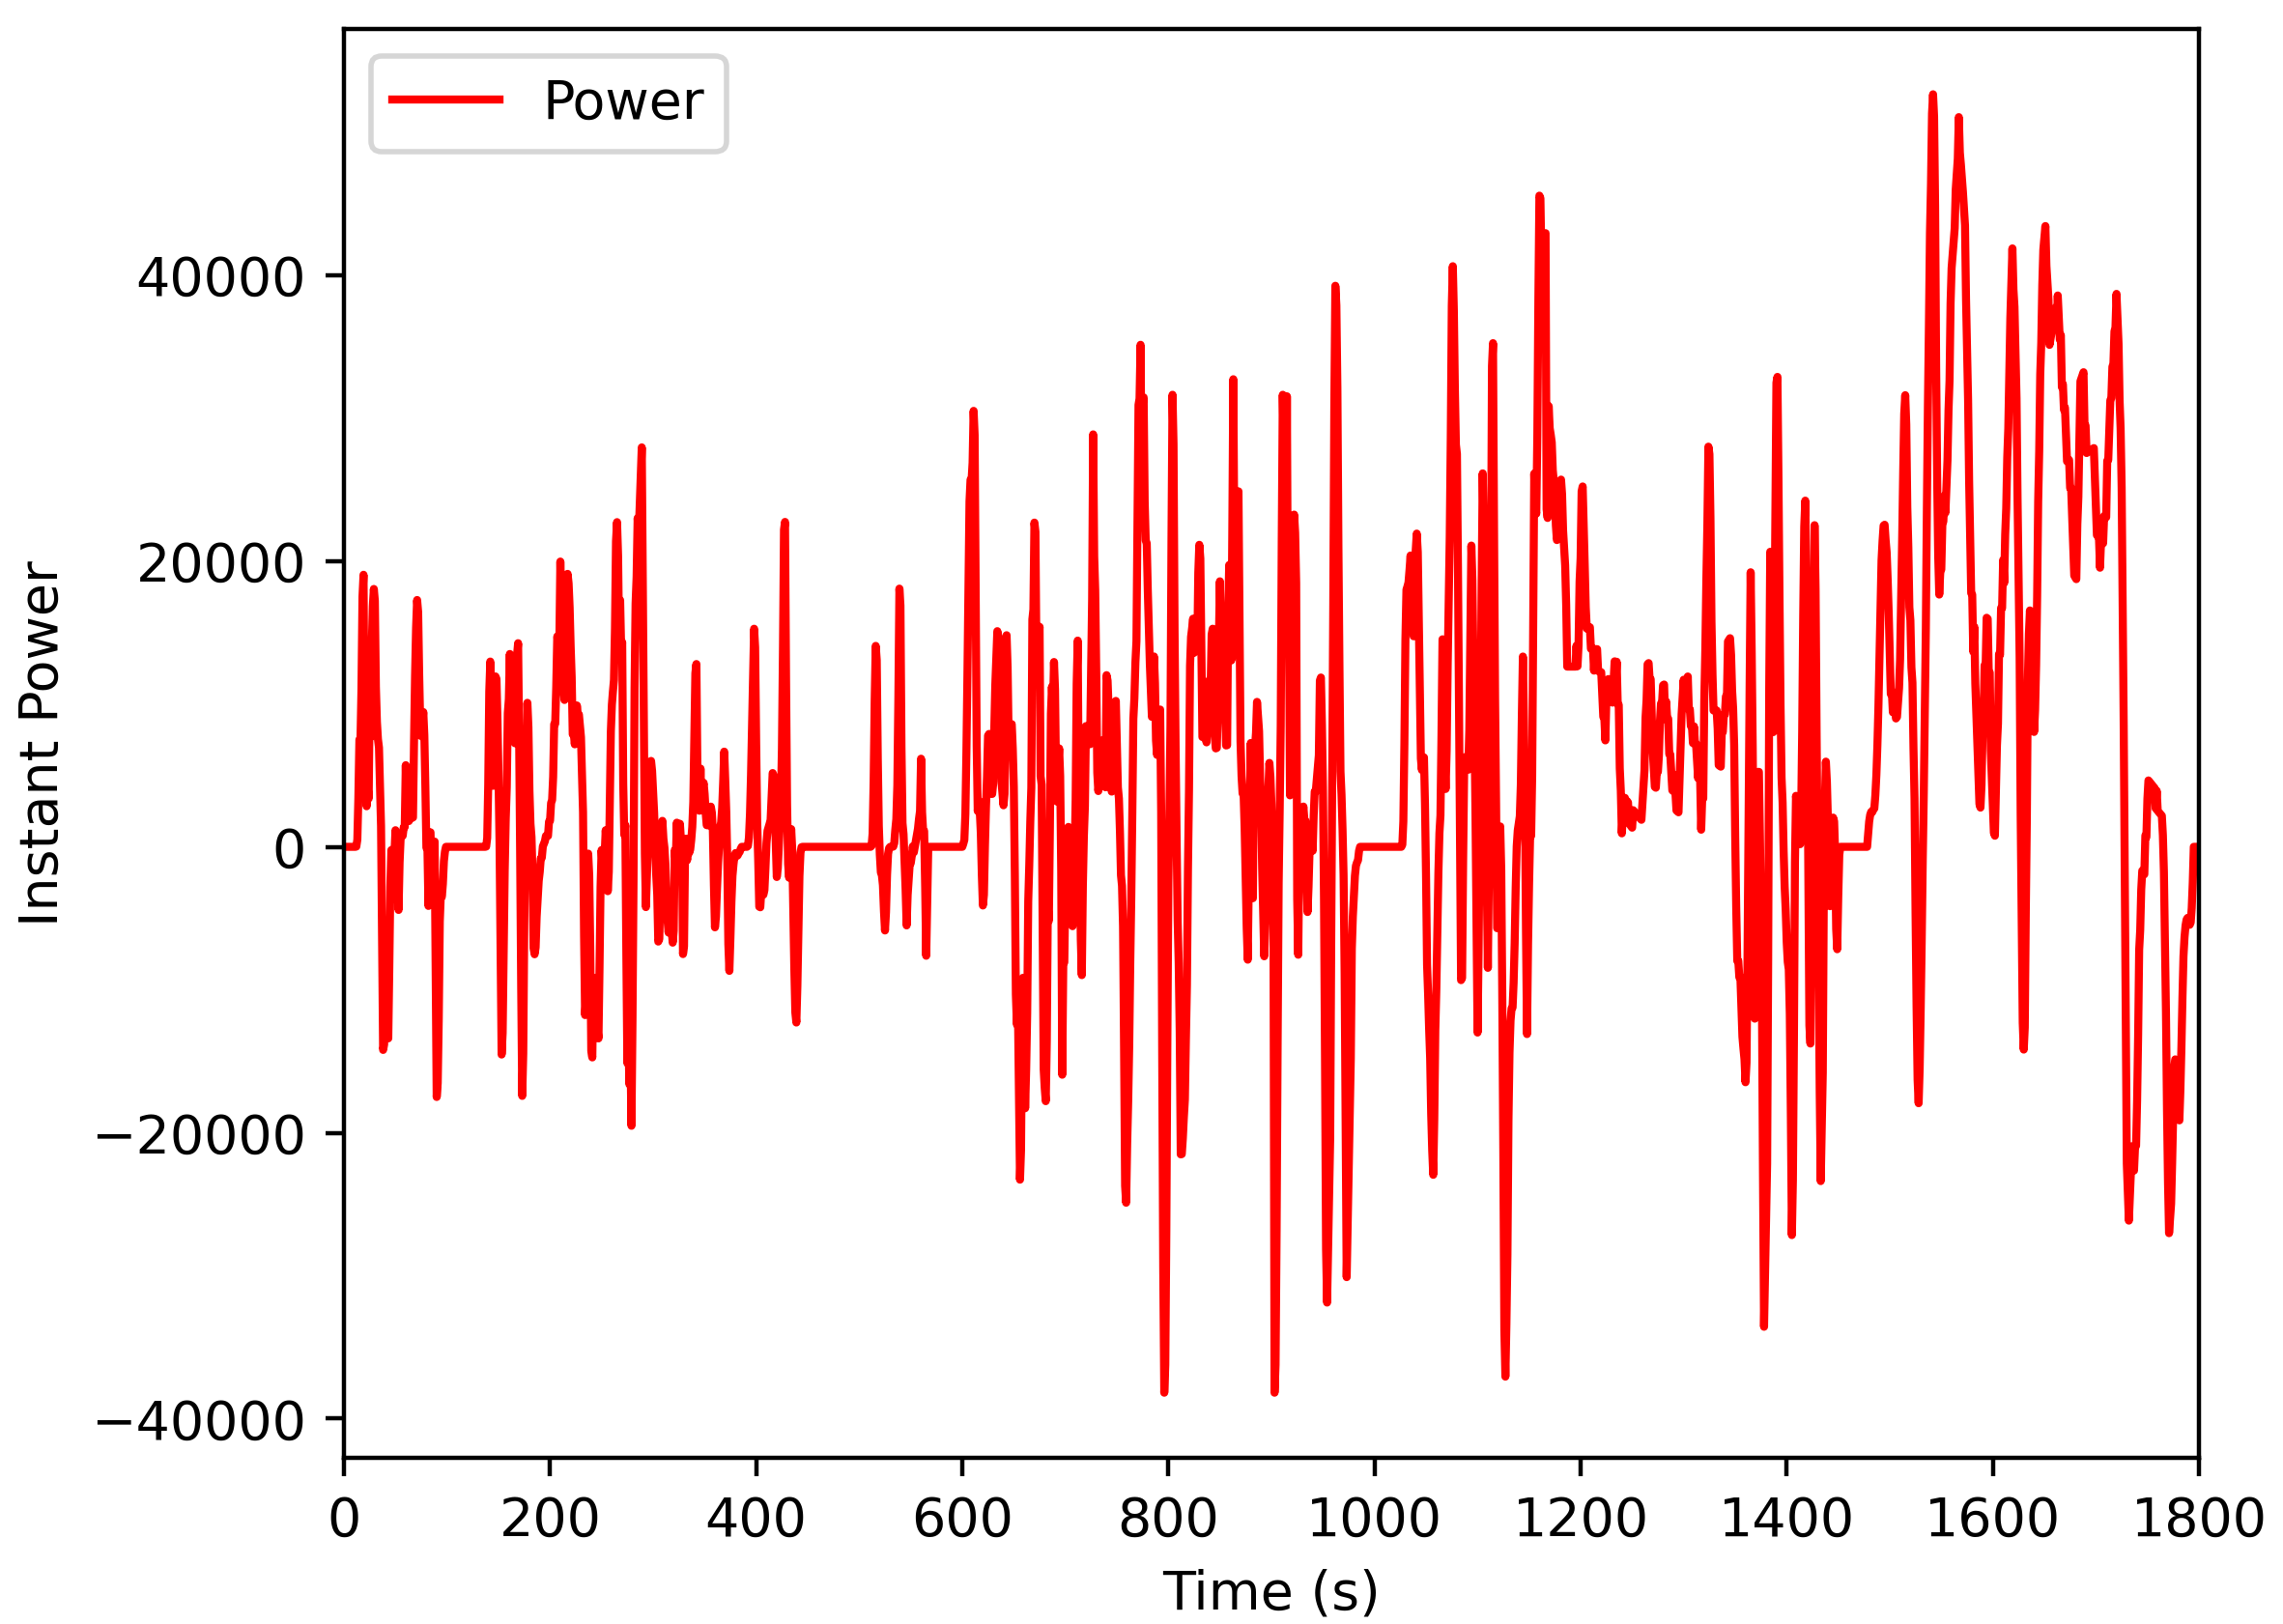
\includegraphics[width=0.7\linewidth]{E:/07. Master_Degree_ITC+UGA/02. ENES3_SGB_UGA/02. New Technology/PEMFC/Power_1.png}
	 	\caption{\small {Instant Power of the Vechicle (W)}}
	 	\label{5}
	 \end{figure}
	
%% ======================================= b . =========================================

	\subsection{Calculate the instant power provide (positive) or received (negative) by the electric hybrid power source. }
	
	The vehicle auxiliaries consume an electrical power of 300W (no air conditioning, minimum consumption of all the equipment of the vehicle: sensor, supervisor,etc.) The DC/DC converter efficiency is assumed constant at 90\% both direction.
	
	\begin{figure}[h]
		\centering 
		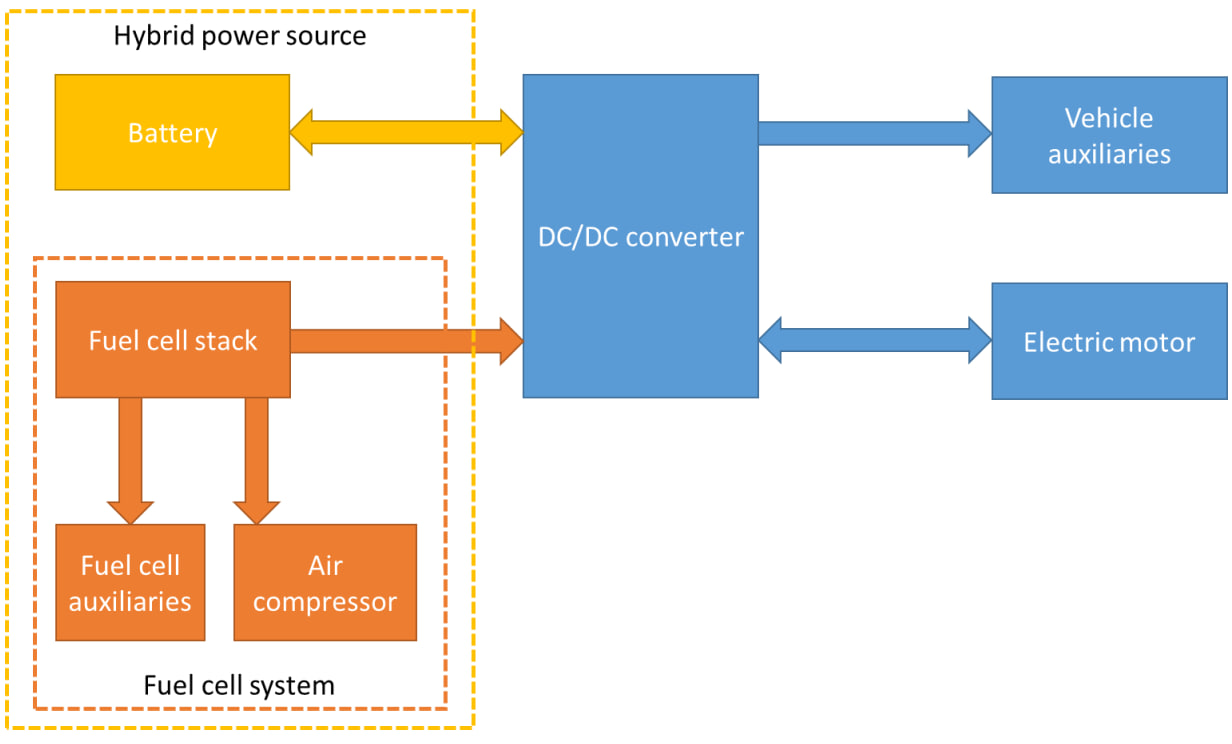
\includegraphics[width=0.8\linewidth]{E:/07. Master_Degree_ITC+UGA/02. ENES3_SGB_UGA/02. New Technology/PEMFC/DC.jpg}
		\caption{\small {Hybrid system in the vehicle}}
		\label{6}
	\end{figure}
\newpage
	\begin{figure}[h]
		\centering 
		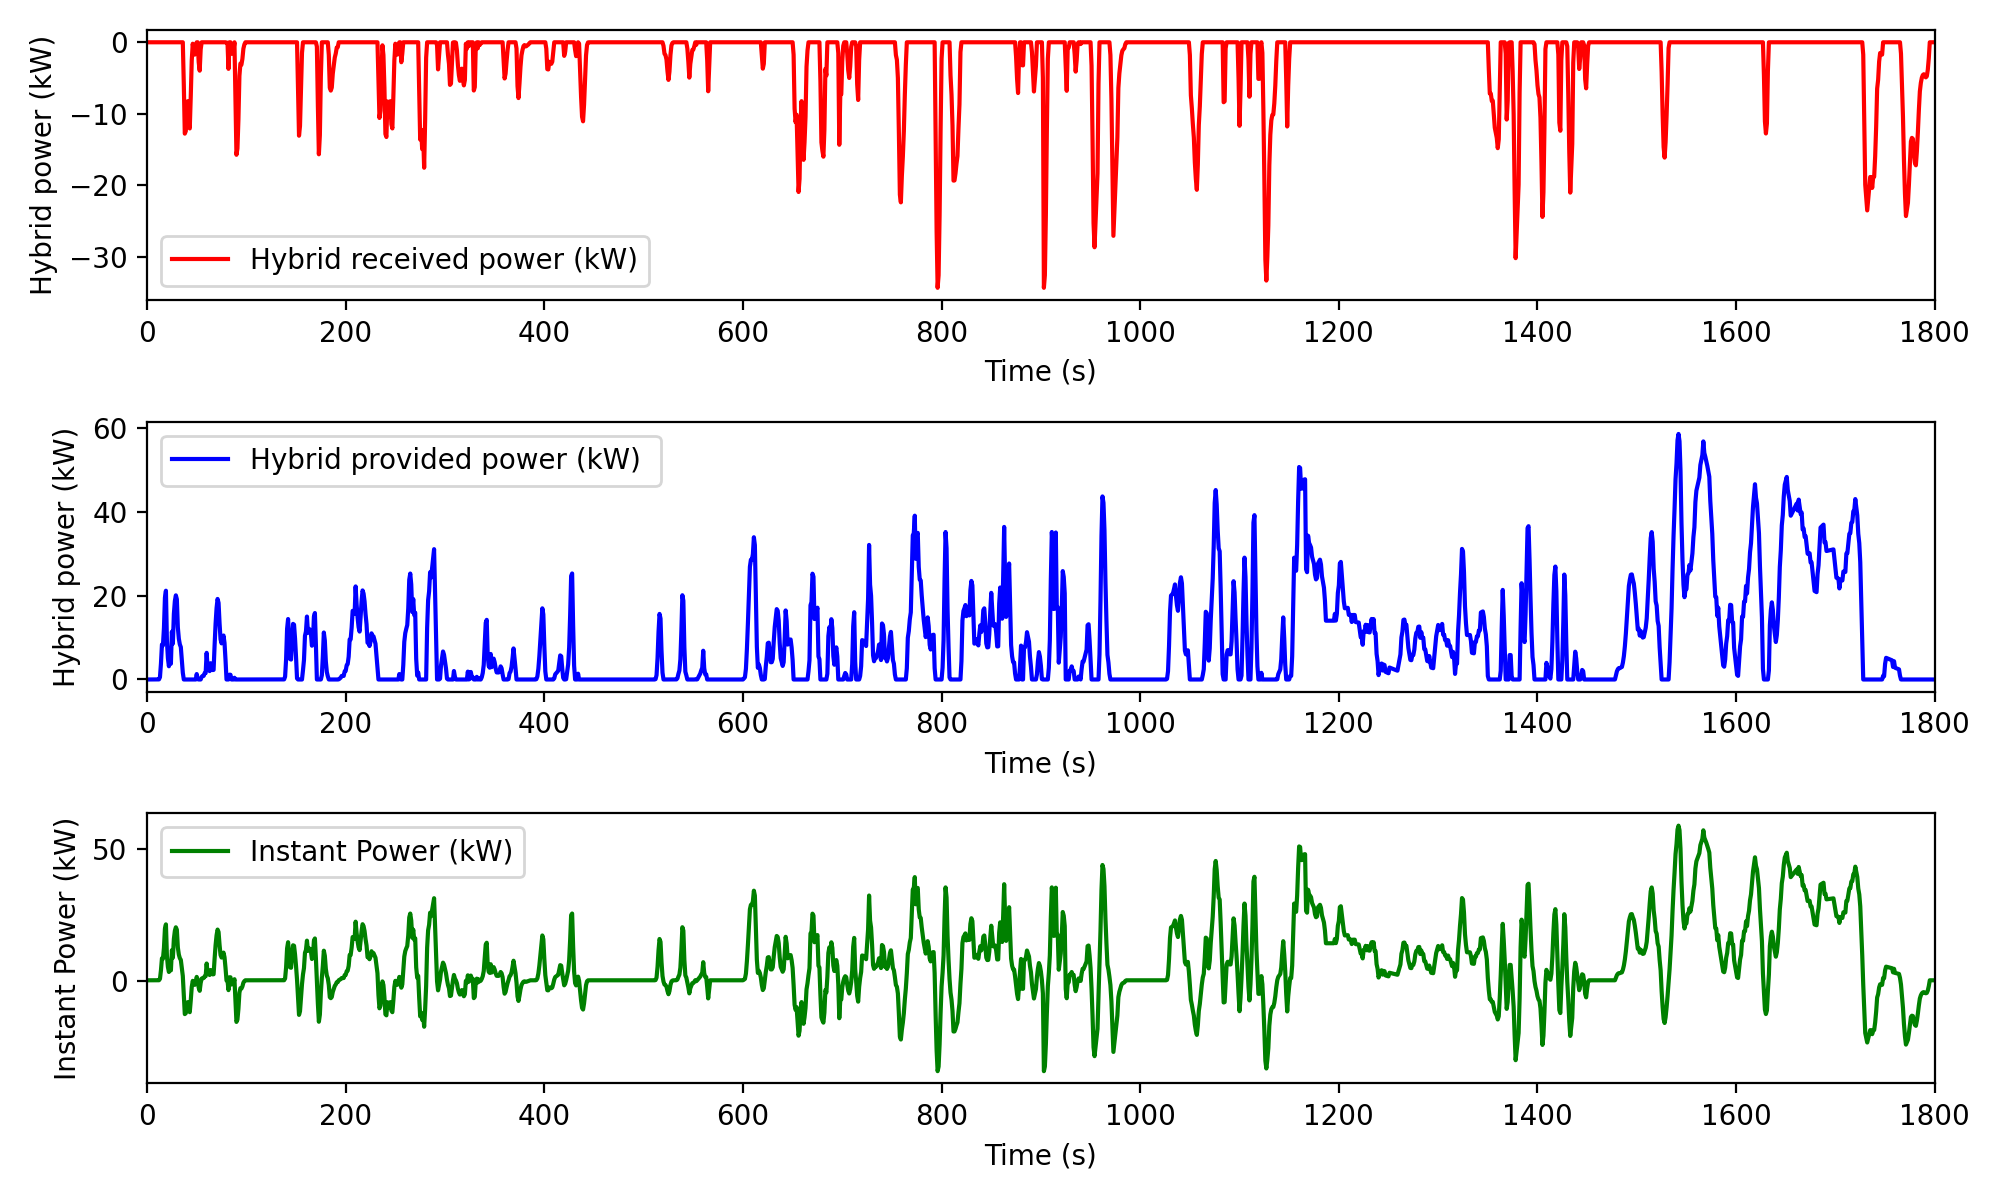
\includegraphics[width=0.95\linewidth]{E:/07. Master_Degree_ITC+UGA/02. ENES3_SGB_UGA/02. New Technology/PEMFC/Question_B.png}
		\caption{\small {Hybrid working system in power transfer}}
		\label{7}
	\end{figure}
	To find the transfer power in the hybrid system in order to find the provided (positive) or recevied (negative), we have use instant power from pervious question as data in the Figure (\ref{5}) with the efficieny of the DC/DC converter. As shown in the Figure (\ref{7}): At the \textbf{first figure} had been show the \textbf{RED line graph} represented the received power (negative) to the hybrid power with the maximum received is \textbf{34.365 kW}. Moreover, as shown in the \textbf{second figure} shown the \textbf{Blue line graph} represented the provided power (positive) from the hybrid system to the motor and auxiliaries. The maximum provided power to the motor was around \textbf{58.488 kW}. According to data from the calculation, we can assumed that the vechicle mostly consum power from the hybrid and less provided power to hybrid system based on the data of speed that provided. 
	
	
	
	
	
	
%% ======================================= c . =========================================





\subsection{Calculate and Plot as a function of time : The power of the battery (kW), The power of the fuel cell system (kW), The SOC battery (\%) }	

The energy management strategy of the hybridization between the battery and the fuel cell system is not disclosed by Tooyta. 
\begin{itemize}
	\item The battery technology is Li-ion, with a stored energy of \textbf{1.24kWh}.
	\item The test results of Mirai 1 indicate that the battery State of Charge (SoC) is comprised between \textbf{50\%} and \textbf{65\%}
	\item The power delivered by the battery is often close to \textbf{5\%} of the total power provided by the hybrid power source when $SoC < 55\%$ or \textbf{30\%} when $SoC > 55\%$
	\item Discharging power of the battery is approximately \textbf{12.4 kW} (or 10C), while the charging power depends on the battery SoC: \textbf{10C} if $SoC < 55\%$ or \textbf{6C} if $SoC > 55\%$
	\item The battery provides $0\%, 5\%, 30\%$ of the total power depending on its SoC and in the limit of its maximum discharging power.
	\item The EMS avoids values of SoC below 50\% and above 65\%
	\item The fuel cell system provides the rest of the power reuqired, excpet if the power demand is too low: the power provided by the fuel cell system can't be lower than \textbf{2.5kW}
\end{itemize}  

	\begin{figure}[h]
	\centering 
	\includegraphics[width=0.95\linewidth]{E:/07. Master_Degree_ITC+UGA/02. ENES3_SGB_UGA/02. New Technology/PEMFC/Question_C.png}
	\caption{\small {Hybrid system, Battery Management, Fuel Cell power and State of Charge in the Vehicle}}
	\label{8}
	\end{figure}

	As the result that shown in the Figure (\ref{8}), 
	\begin{itemize}
		\item The first plot of the Figure (\ref{8}) (represented by the by blue curve) show about the \textbf{Hybrid Power} working in the system.
		\item The second plot of the Figure (\ref{8}) (represented by the by yellow curve) show the characteristic of the charging and discharging of the Battery in the vehicle. The maximum power discharging is \textbf{12.4 kW} and the maximum power charging is \textbf{7.44 kW}. The status of charge and discharge ws depend on the time and speed per second.
		\item  The third plot of the Figure (\ref{8}) (represented by the by green curve) show the fuel cell consumption that will be use in the system. The maximum fuel cell consumption is \textbf{46.42 kW}. The consumption of the fuel cell variable depend on the time.
		\item The fourth plot in Figure (\ref{8}) (represented by the by red curve) illustrates the State of Charge (SoC) of the battery system. By using formula to determine State of Charge in the system, we do it by : 
	\begin{equation}
			\text{SoC}_i = \min\left( \text{SoC}_{\text{max}}, \max\left( \text{SoC}_{\text{min}}, \text{SoC}_{i-1} - \frac{\text{power bat}_i}{3600 \cdot \text{batcapacity}} + \frac{\text{demand}_i}{3600 \cdot \text{batcapacity}} \right) \right)
	\end{equation}

		
		It starts with an initial SoC of approximately \textbf{60\%} and gradually decreases to \textbf{56.28\%} over time, depending on the driving characteristics. The SoC can fluctuate, increasing or decreasing based on the motor's operation and the dynamics of the hybrid system.
		
	\end{itemize}


%% ======================================= d . =========================================

\subsection{Make the same analysis with the road cycle "130 kmh". Consider two different cases : $\alpha = 0^\circ$ and $\alpha = 2^\circ$ } 
	
	\subsubsection{Analysis $\alpha = 0^\circ$}
		\begin{figure}[h]
			\centering 
			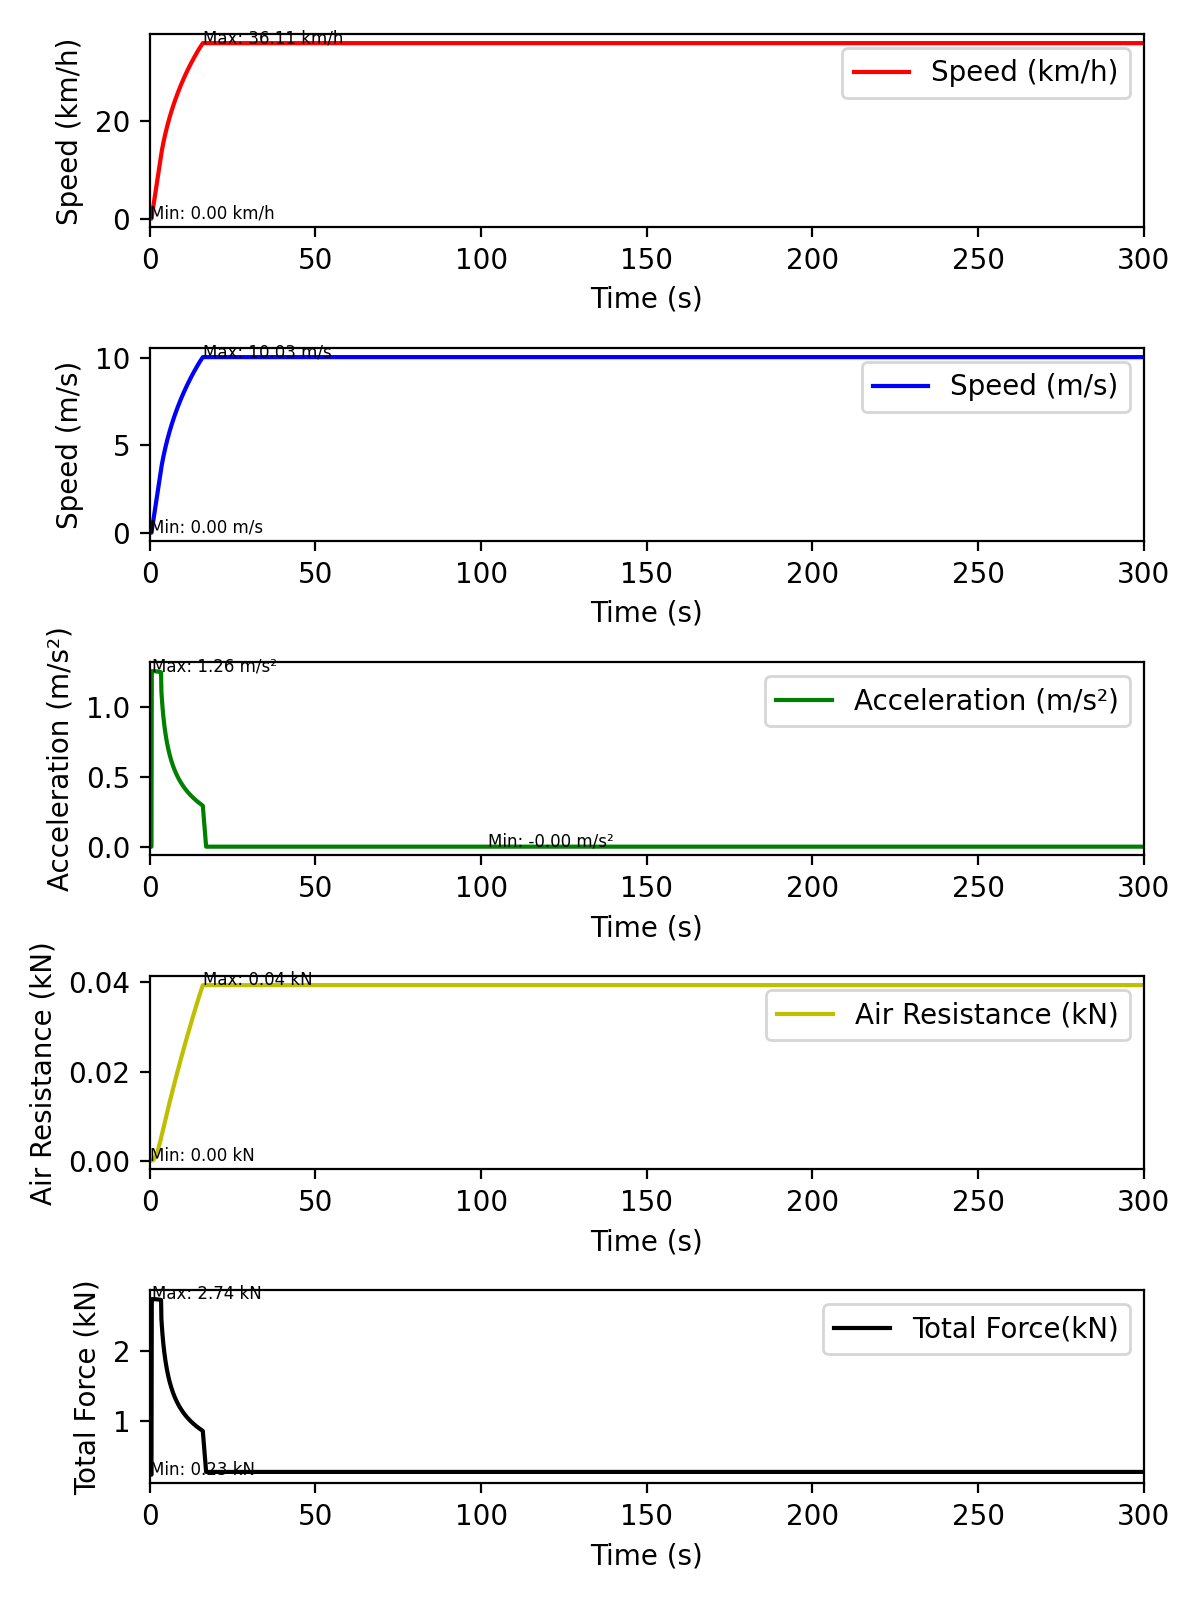
\includegraphics[width=0.83\linewidth]{E:/07. Master_Degree_ITC+UGA/02. ENES3_SGB_UGA/02. New Technology/PEMFC/Question_A_130.png}
			\caption{\small {Plots related to Speed, acceleration, air resistance, and Total Force over time}}
			\label{9}
		\end{figure}

	In the Figure (\ref{9}), it was shown the data curve about the speed within $km/h$ and $m/s$, acceleration in $m/s^2$, Air Resistance and Rolling Resistance.

\begin{itemize}
	\item The first red and blue curve in the Figure (\ref{9}) represented to the speed of the vehicle drive over time in $km/h$ and $m/s$.
	\item The green curve in the Figure (\ref{9}) presented to the acceleration of the vehicle that show the characteristic of the vehicle drive. (Increase or Decrease Speed)
	\item The air resistance calculated by using Equation (\ref{eq1})  and (\ref{eq8}) . The result of the calculate shown in the yellow curve of the Figure (\ref{9}).
	\item The total Force or Motor Force determined by usig Equation (\ref{eq5}) and the result of the calculation displayed at the black curve shown that the maximum motor force is \textbf{2.74 kN}.
\end{itemize}


\begin{figure}[h]
	\centering 
	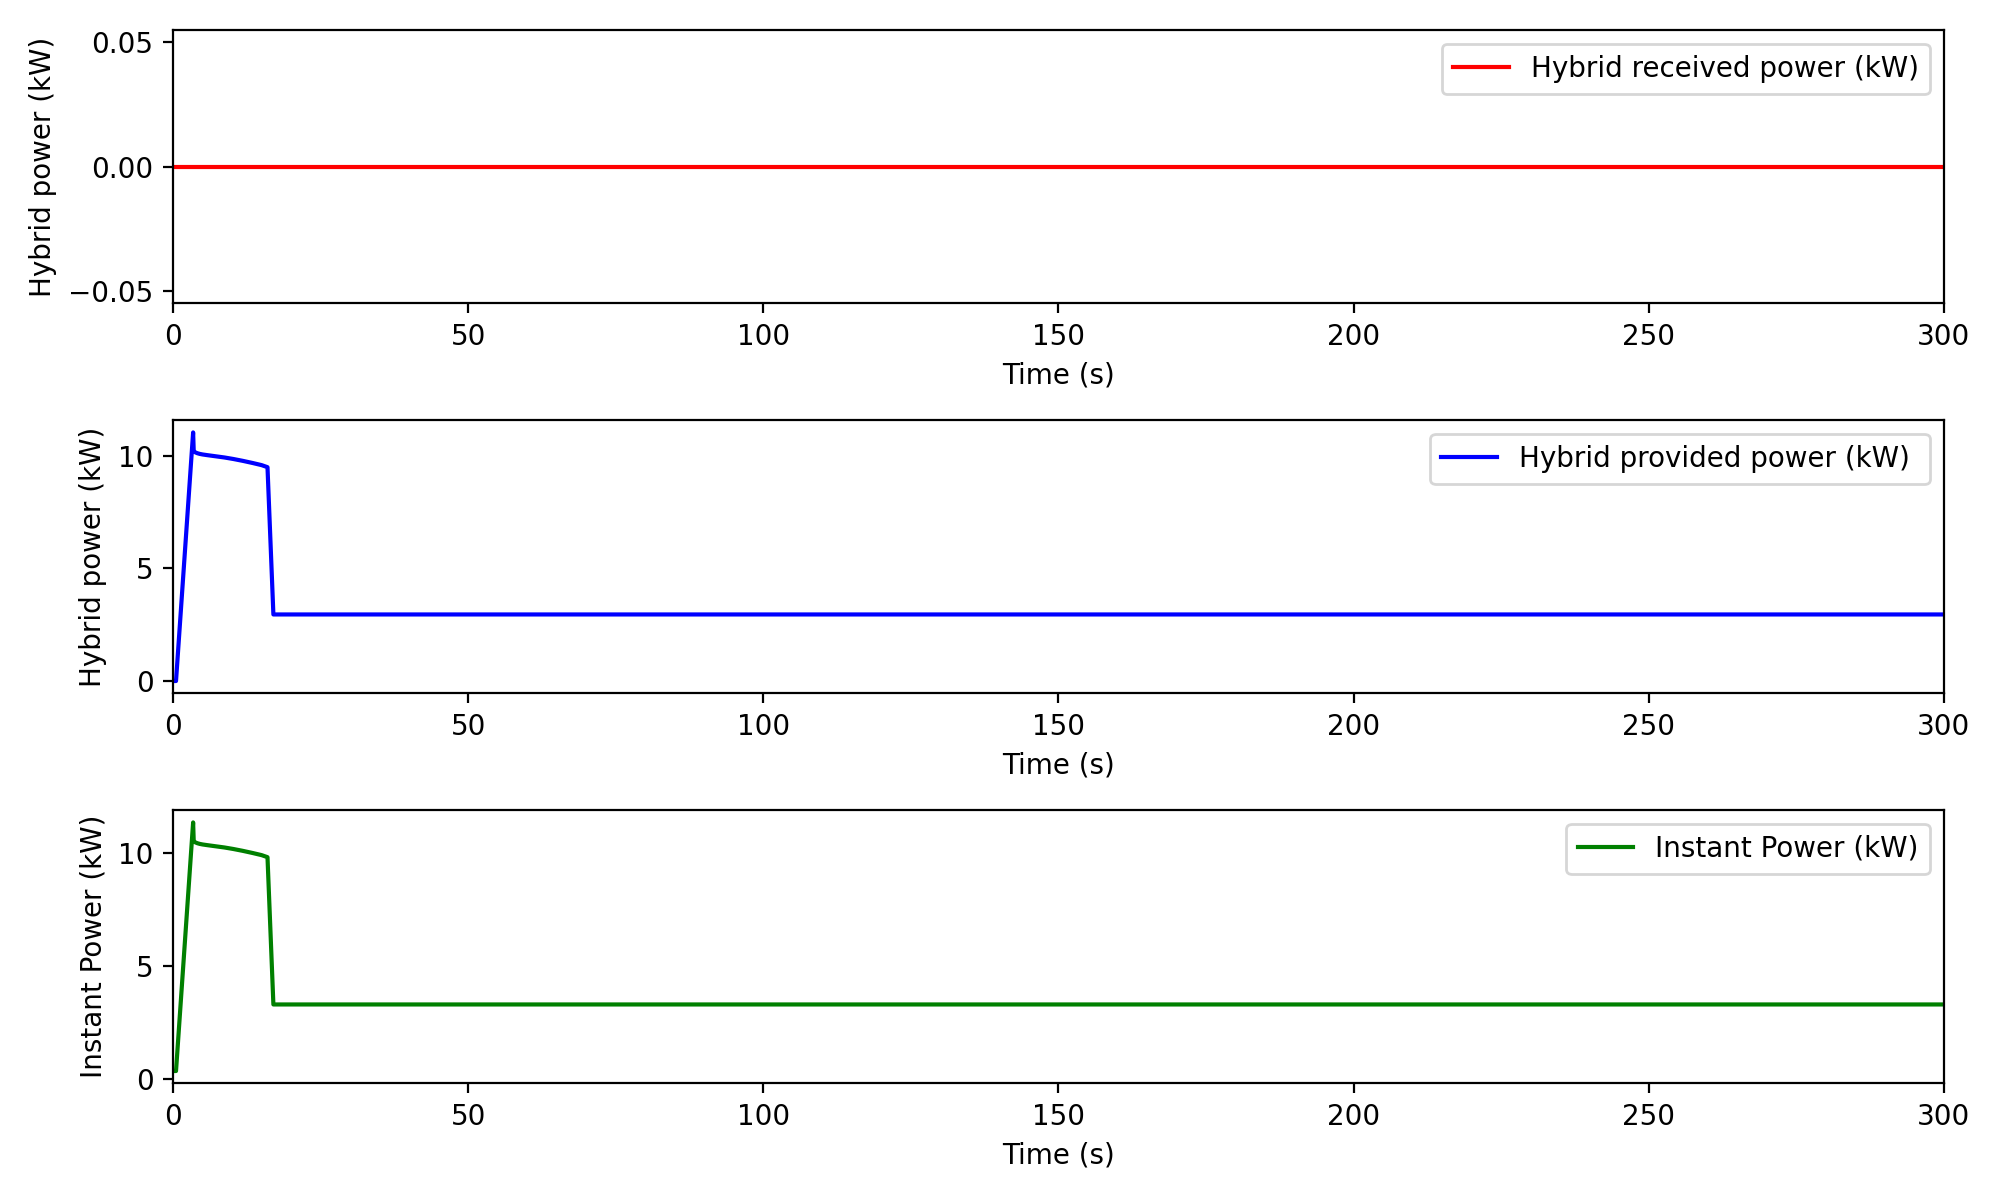
\includegraphics[width=0.9\linewidth]{E:/07. Master_Degree_ITC+UGA/02. ENES3_SGB_UGA/02. New Technology/PEMFC/Question_B_130.png}
	\caption{\small {Hybrid working in Power transfer in Vehicle 130kmh}}
	\label{10}
\end{figure}
As show in Figure (\ref{10}), we can assume that vehicle at this speed characteristic shown that the Hybrid system did not receive any power from the motor but it provided full power to the motor.


\begin{figure}[h]
	\centering 
	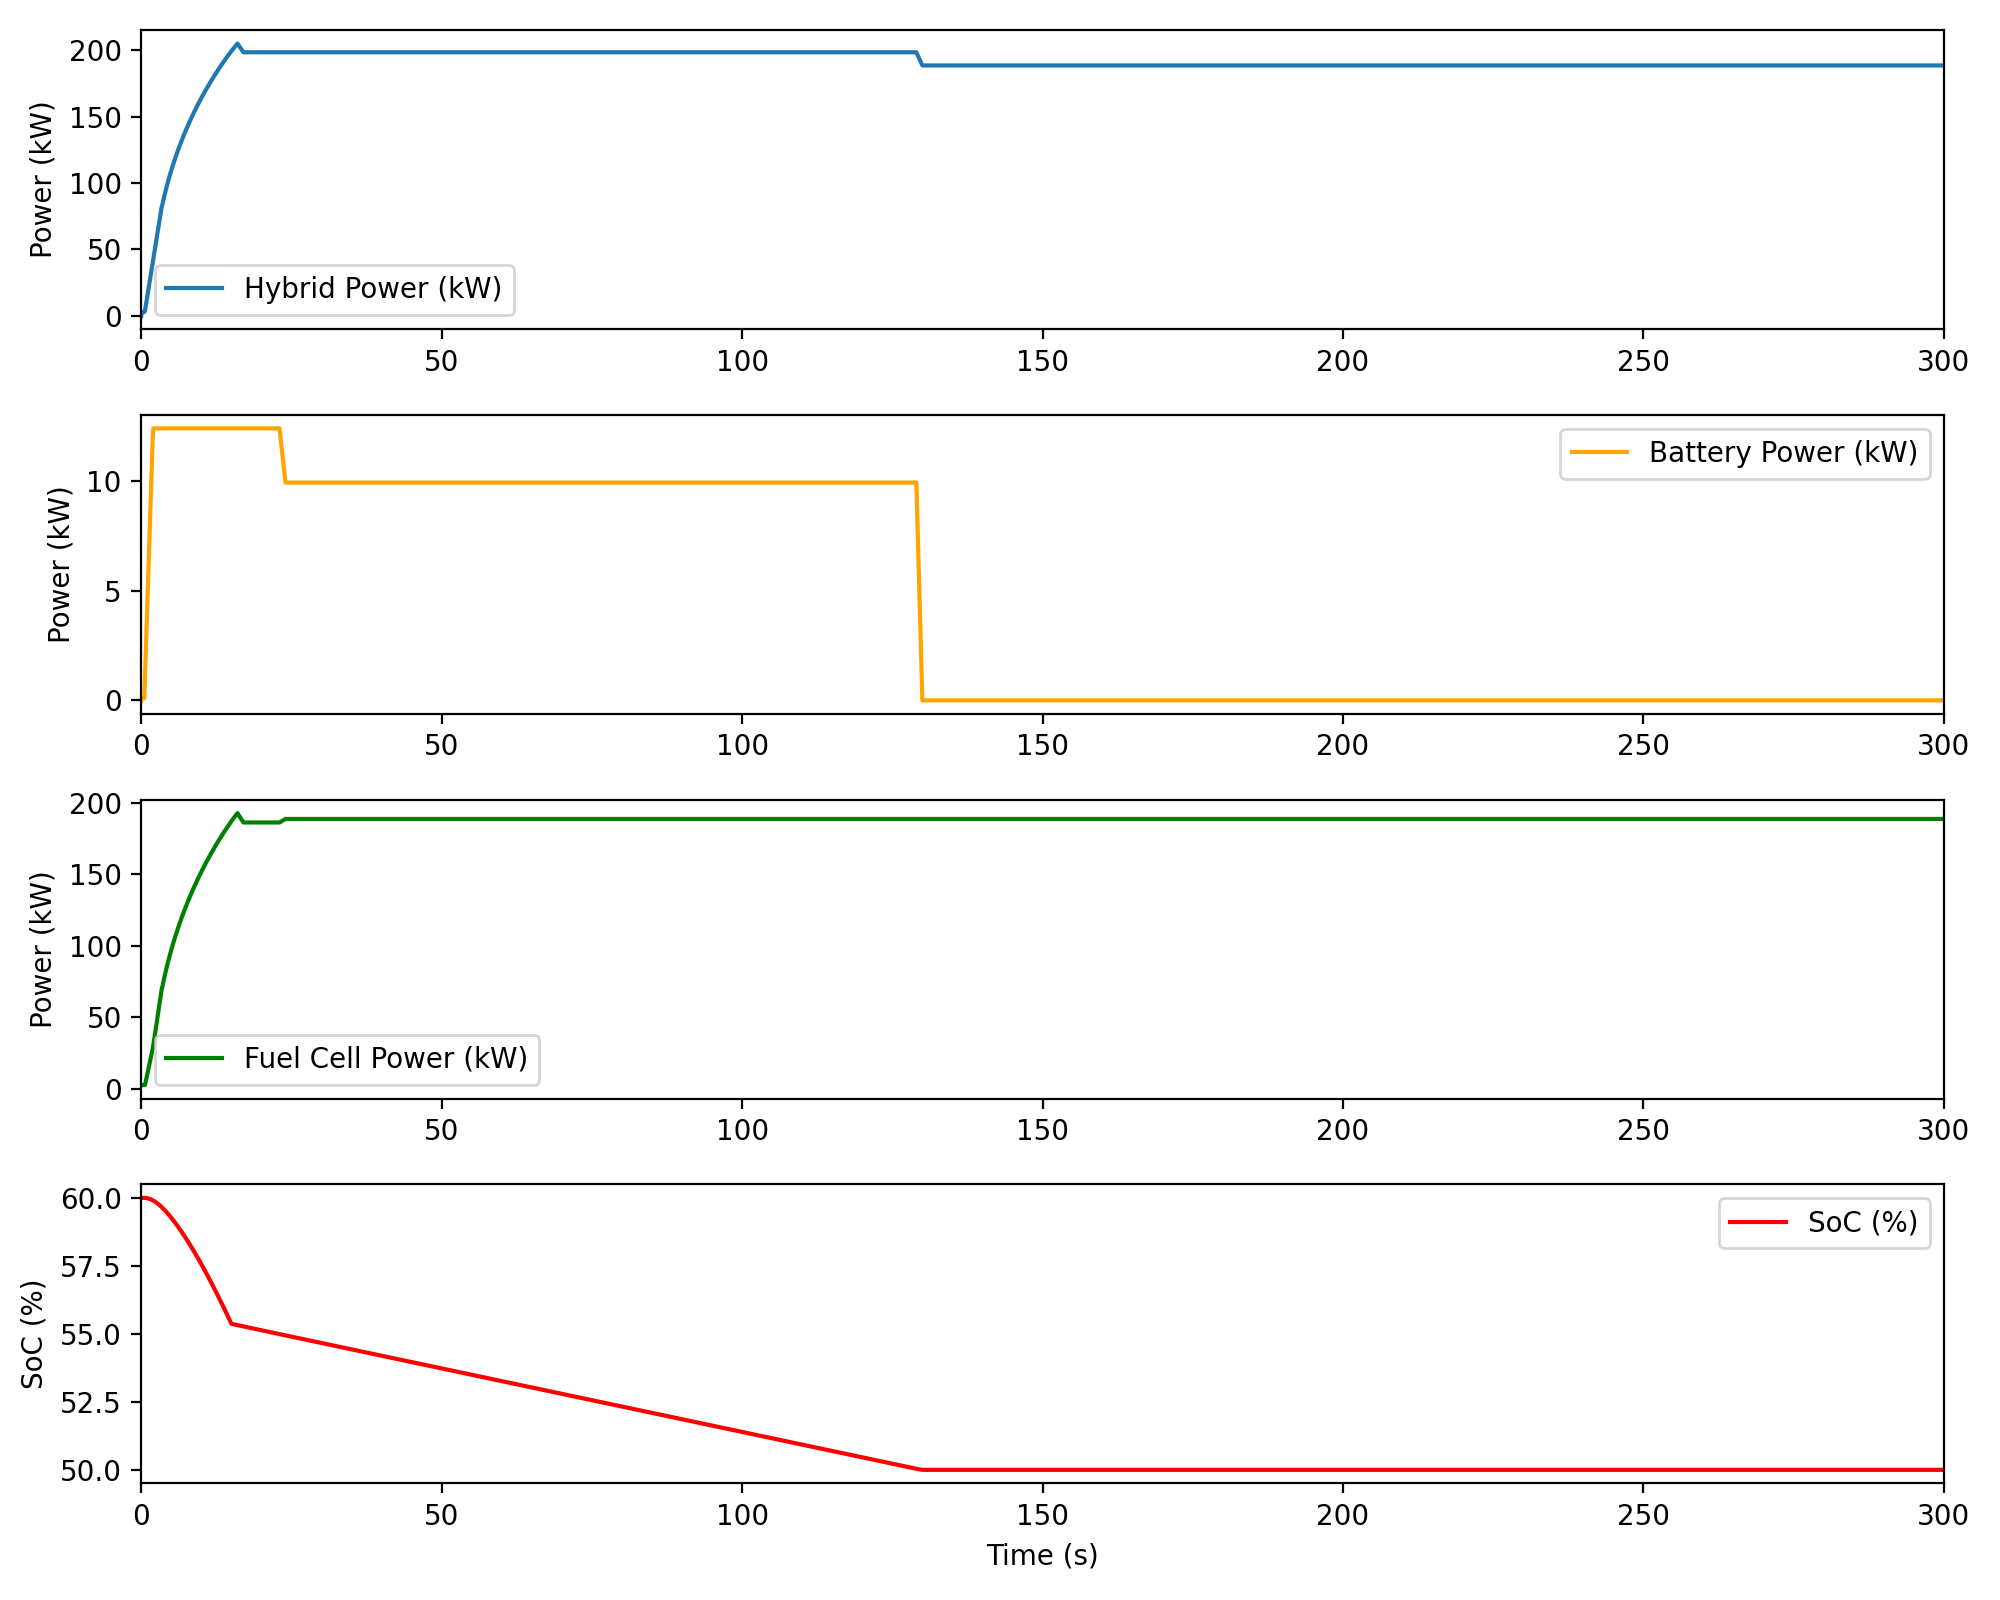
\includegraphics[width=0.9\linewidth]{E:/07. Master_Degree_ITC+UGA/02. ENES3_SGB_UGA/02. New Technology/PEMFC/Question_C_130.png}
	\caption{\small {Hybrid system, Battery Management, Fuel Cell power and State of Charge in the Vehicle}}
	\label{11}
\end{figure}
\begin{itemize}
	\item \textbf{Hybrid Power (kW)}:
	\begin{itemize}
		\item This plot shows the total hybrid power delivered by the system.
		\item The power reaches a peak of approximately 3.17 kW at the start.
		\item It rapidly drops to 0 kW after around 25 seconds and remains flat for the rest of the 300-second period.
	\end{itemize}
	
	\item \textbf{Battery Power (kW)}:
	\begin{itemize}
		\item This plot shows the power supplied by the battery alone.
		\item Initially, the battery power spikes to a peak of around 3.31 kW.
		\item It sharply decreases to 0 kW after about 25 seconds, staying at that level for the rest of the duration.
	\end{itemize}
	
	\item \textbf{Fuel Cell Power (kW)}:
	\begin{itemize}
		\item This plot shows the power generated by the fuel cell.
		\item The fuel cell power reaches a maximum of about 2.76 kW early in the period.
		\item It drops rapidly to 2.5 kW within 25 seconds and remains constant at this level for the remainder of the time.
	\end{itemize}
	
	\item \textbf{State of Charge (SoC) (\%)}:
	\begin{itemize}
		\item This plot represents the battery’s state of charge (SoC) over time.
		\item The SoC starts at approximately 60\% and decreases gradually over time.
		\item By the end of the 300-second period, it reaches around 59.3\%.
	\end{itemize}
\end{itemize}




% ======================================C .  ALPHA 2 =====================================================\\

\subsubsection{Analysis $\alpha = 2^\circ$}


\begin{figure}[h]
	\centering 
	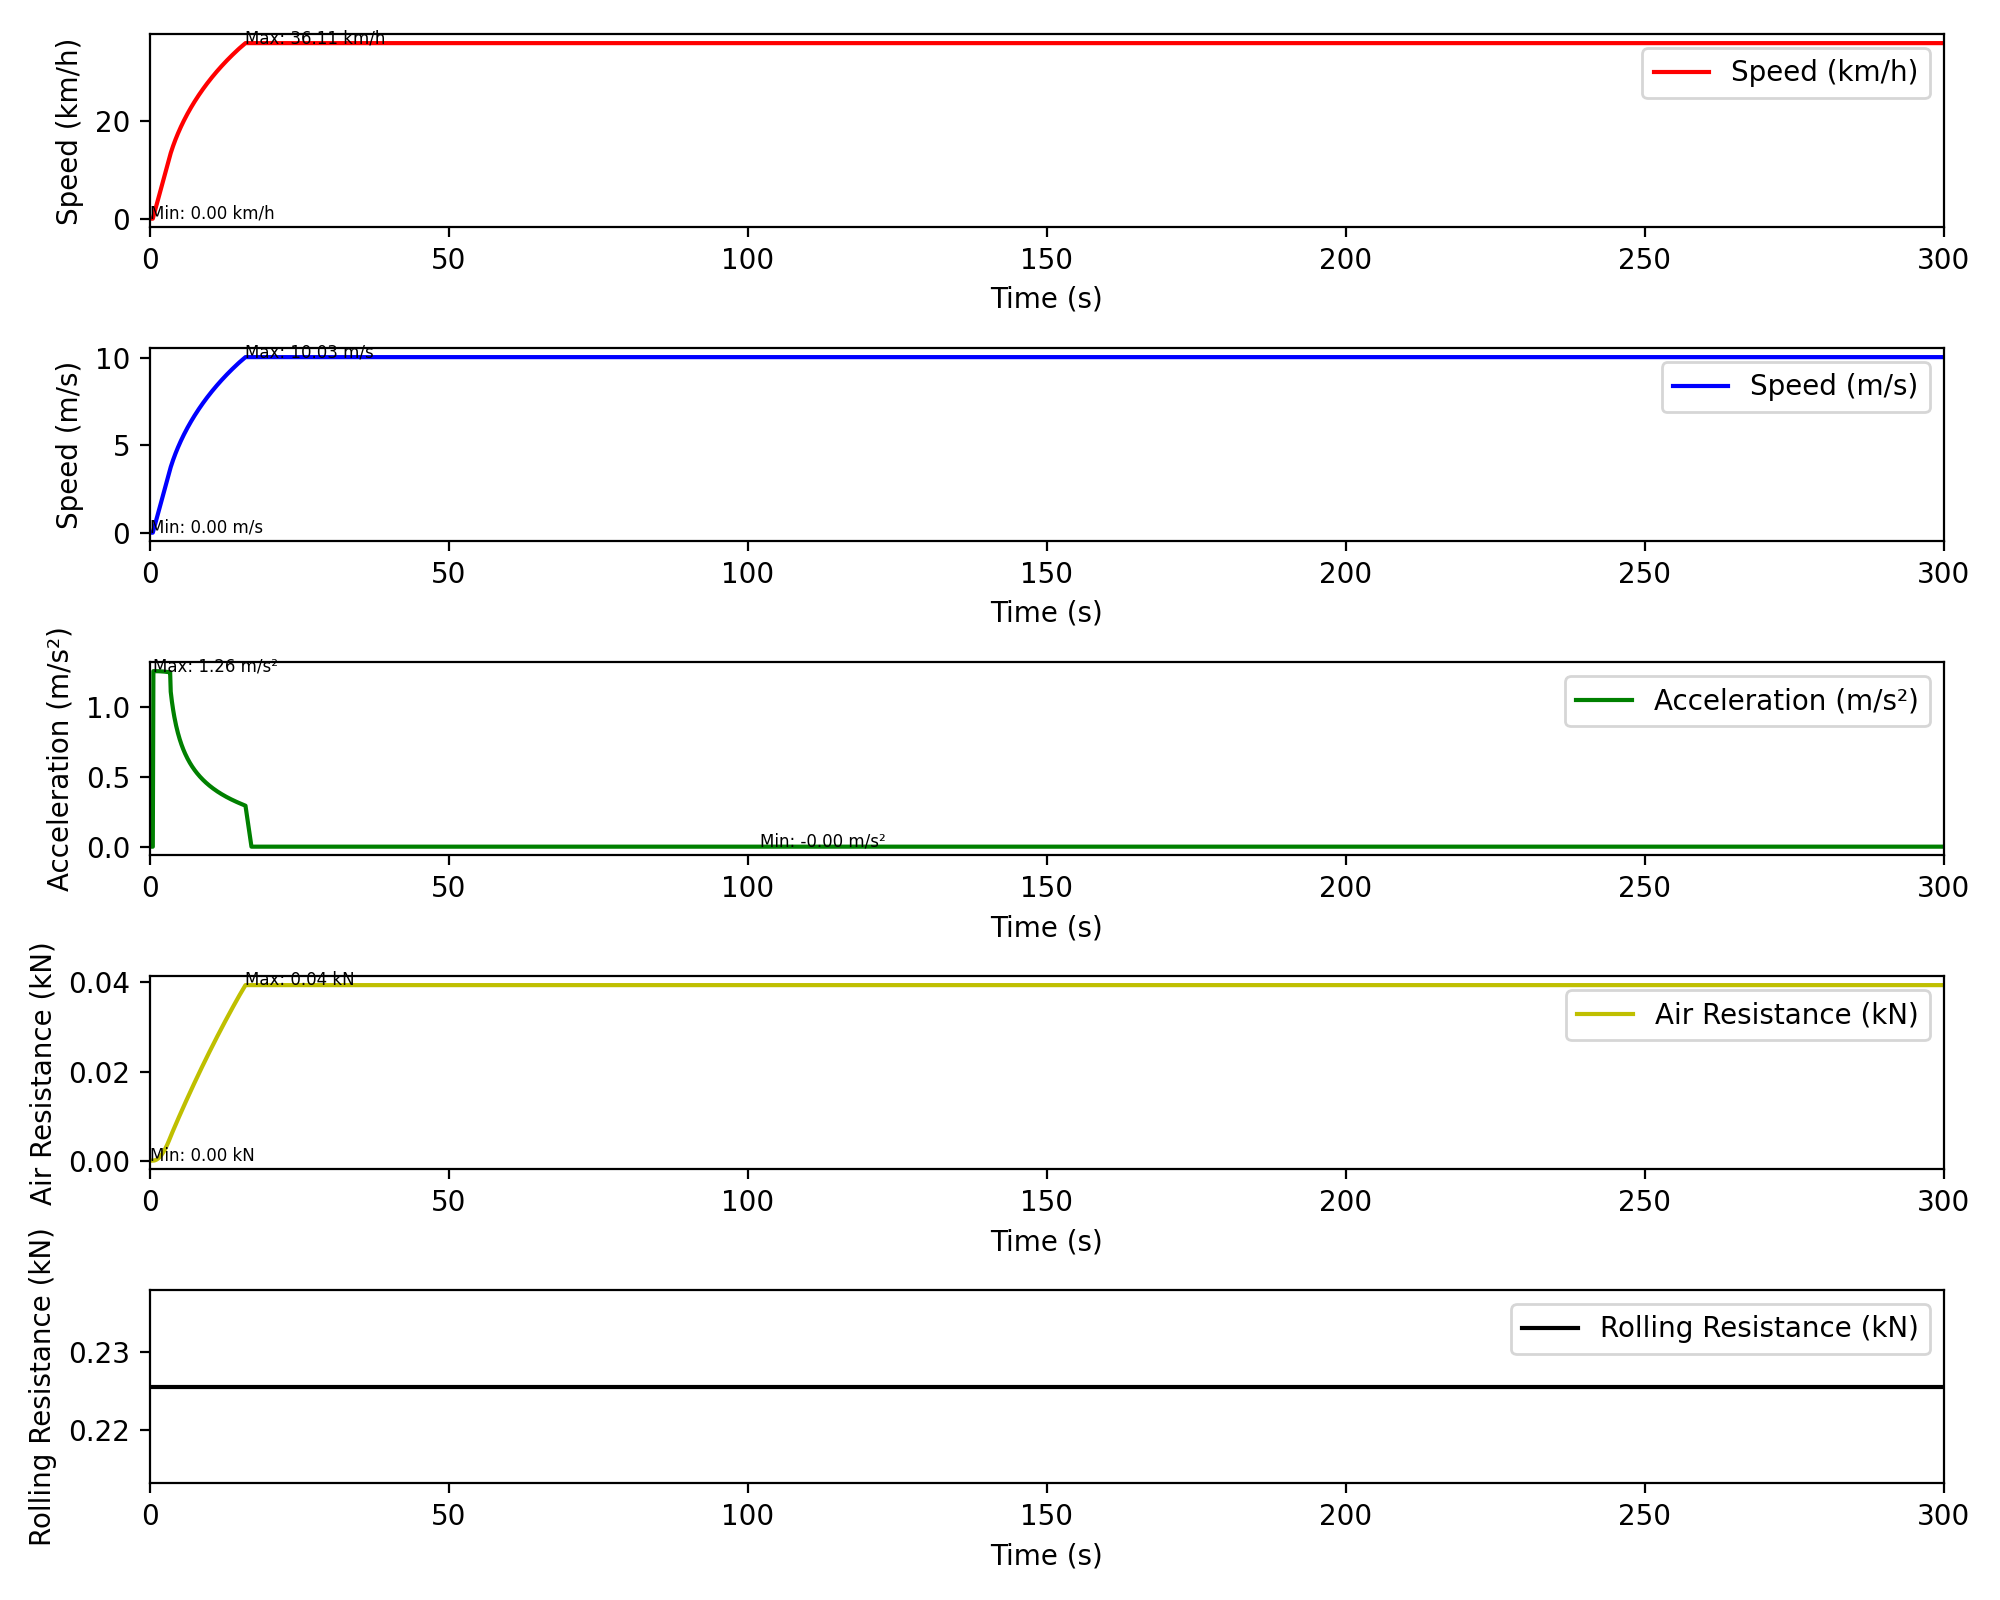
\includegraphics[width=0.87\linewidth]{E:/07. Master_Degree_ITC+UGA/02. ENES3_SGB_UGA/02. New Technology/PEMFC/Question_A_130_V2.png}
	\caption{\small {Plots related to Speed, acceleration, air resistance, and Total Force over time}}
	\label{12}
\end{figure}

The speed and acceleration are the same from the pervious but there are some change on the air resistance, rolling resistance and climbing	resistance. 

\begin{itemize}
	\item For the Air resistance using Equation (\ref{eq1}), we got the result shown in the Figure (\ref{12}).
	\item The Rolling Resistance using Equation (\ref{eq2}), as the result we can write :
	\begin{equation}
		F_{rolling}(t) = 200kg\times9.81m/s^2\times0.0115\times \cos(0^\circ) = \textbf{225.4926 N}\label{eq13}
	\end{equation}
	\item The Climbing Resistance using Equation (\ref{eq3}), as the result we computed :
	\begin{equation}
		F_{climb}(t) = Mg\sin(\alpha) = 2000kg \times 9.81m/s^2 \times \sin(2^\circ) = \textbf{684.811 N} \label{eq14}
	\end{equation}
	\item The total Force or Motor Force determined by usig Equation (\ref{eq5}) and the result of the calculation displayed at the black curve shown that the maximum motor force is \textbf{3.43 kN}.
\end{itemize}


\begin{figure}[h]
	\centering 
	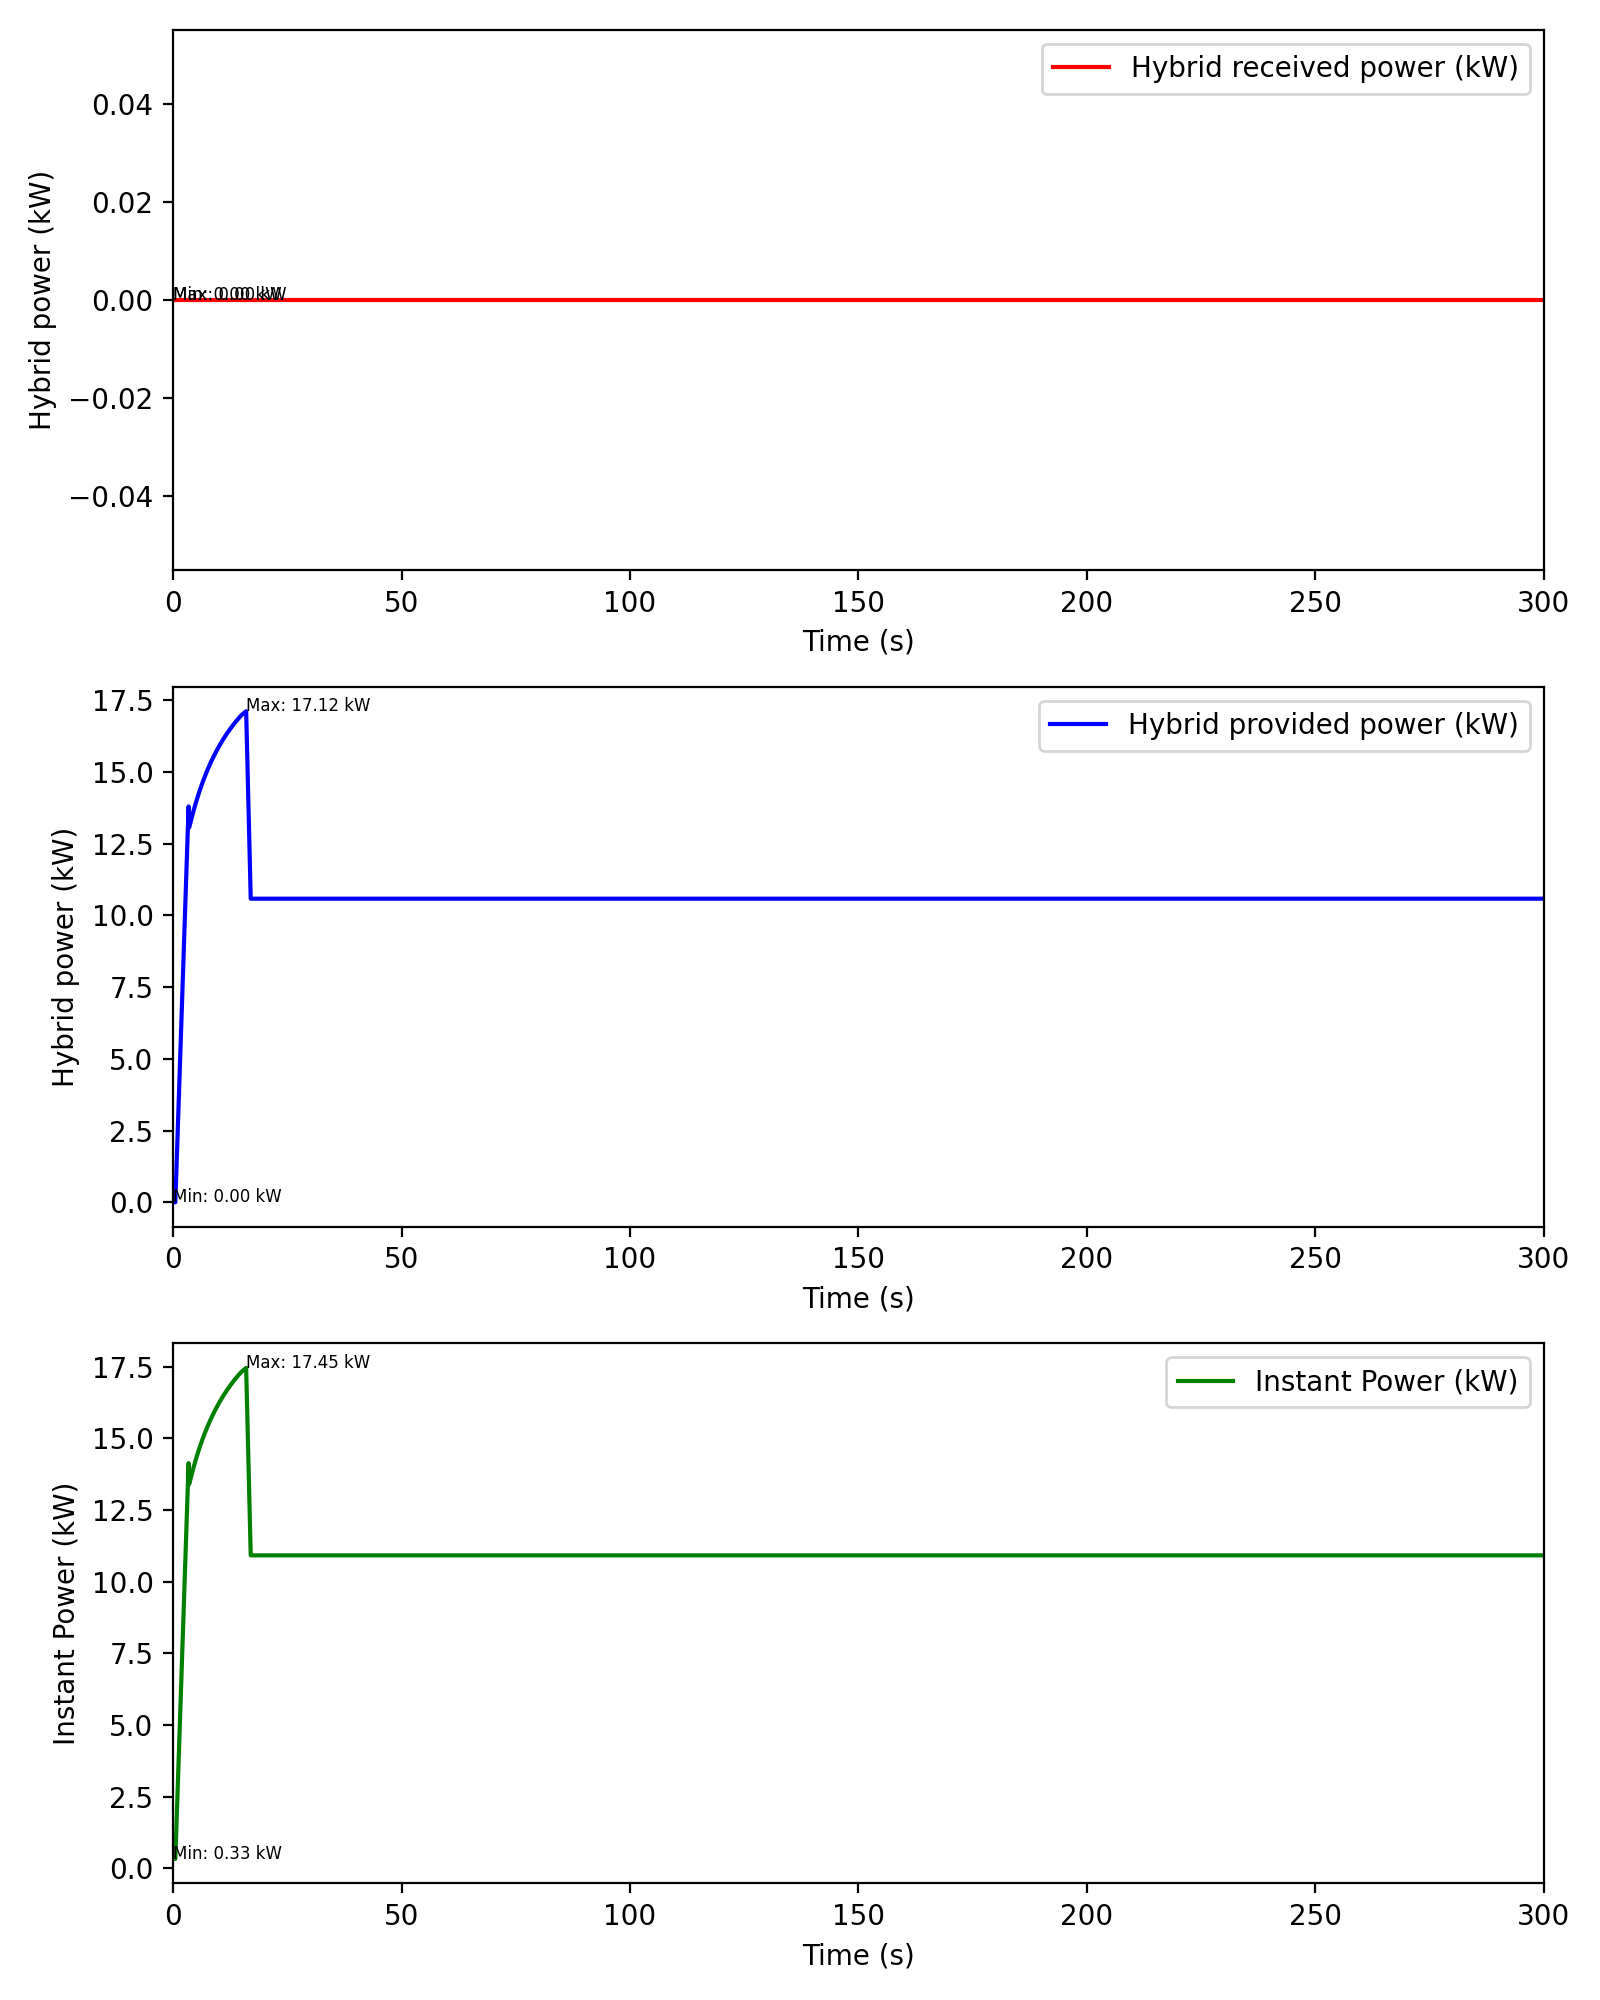
\includegraphics[width=0.83\linewidth]{E:/07. Master_Degree_ITC+UGA/02. ENES3_SGB_UGA/02. New Technology/PEMFC/Question_B_130_V2.png}
	\caption{\small {Hybrid working in Power transfer in Vehicle 130kmh}}
	\label{13}
\end{figure}

As show in Figure (\ref{13}), we can assume that vehicle at this speed characteristic shown that the Hybrid system did not receive any power from the motor but it provided full power to the motor.

\begin{figure}[h]
	\centering 
	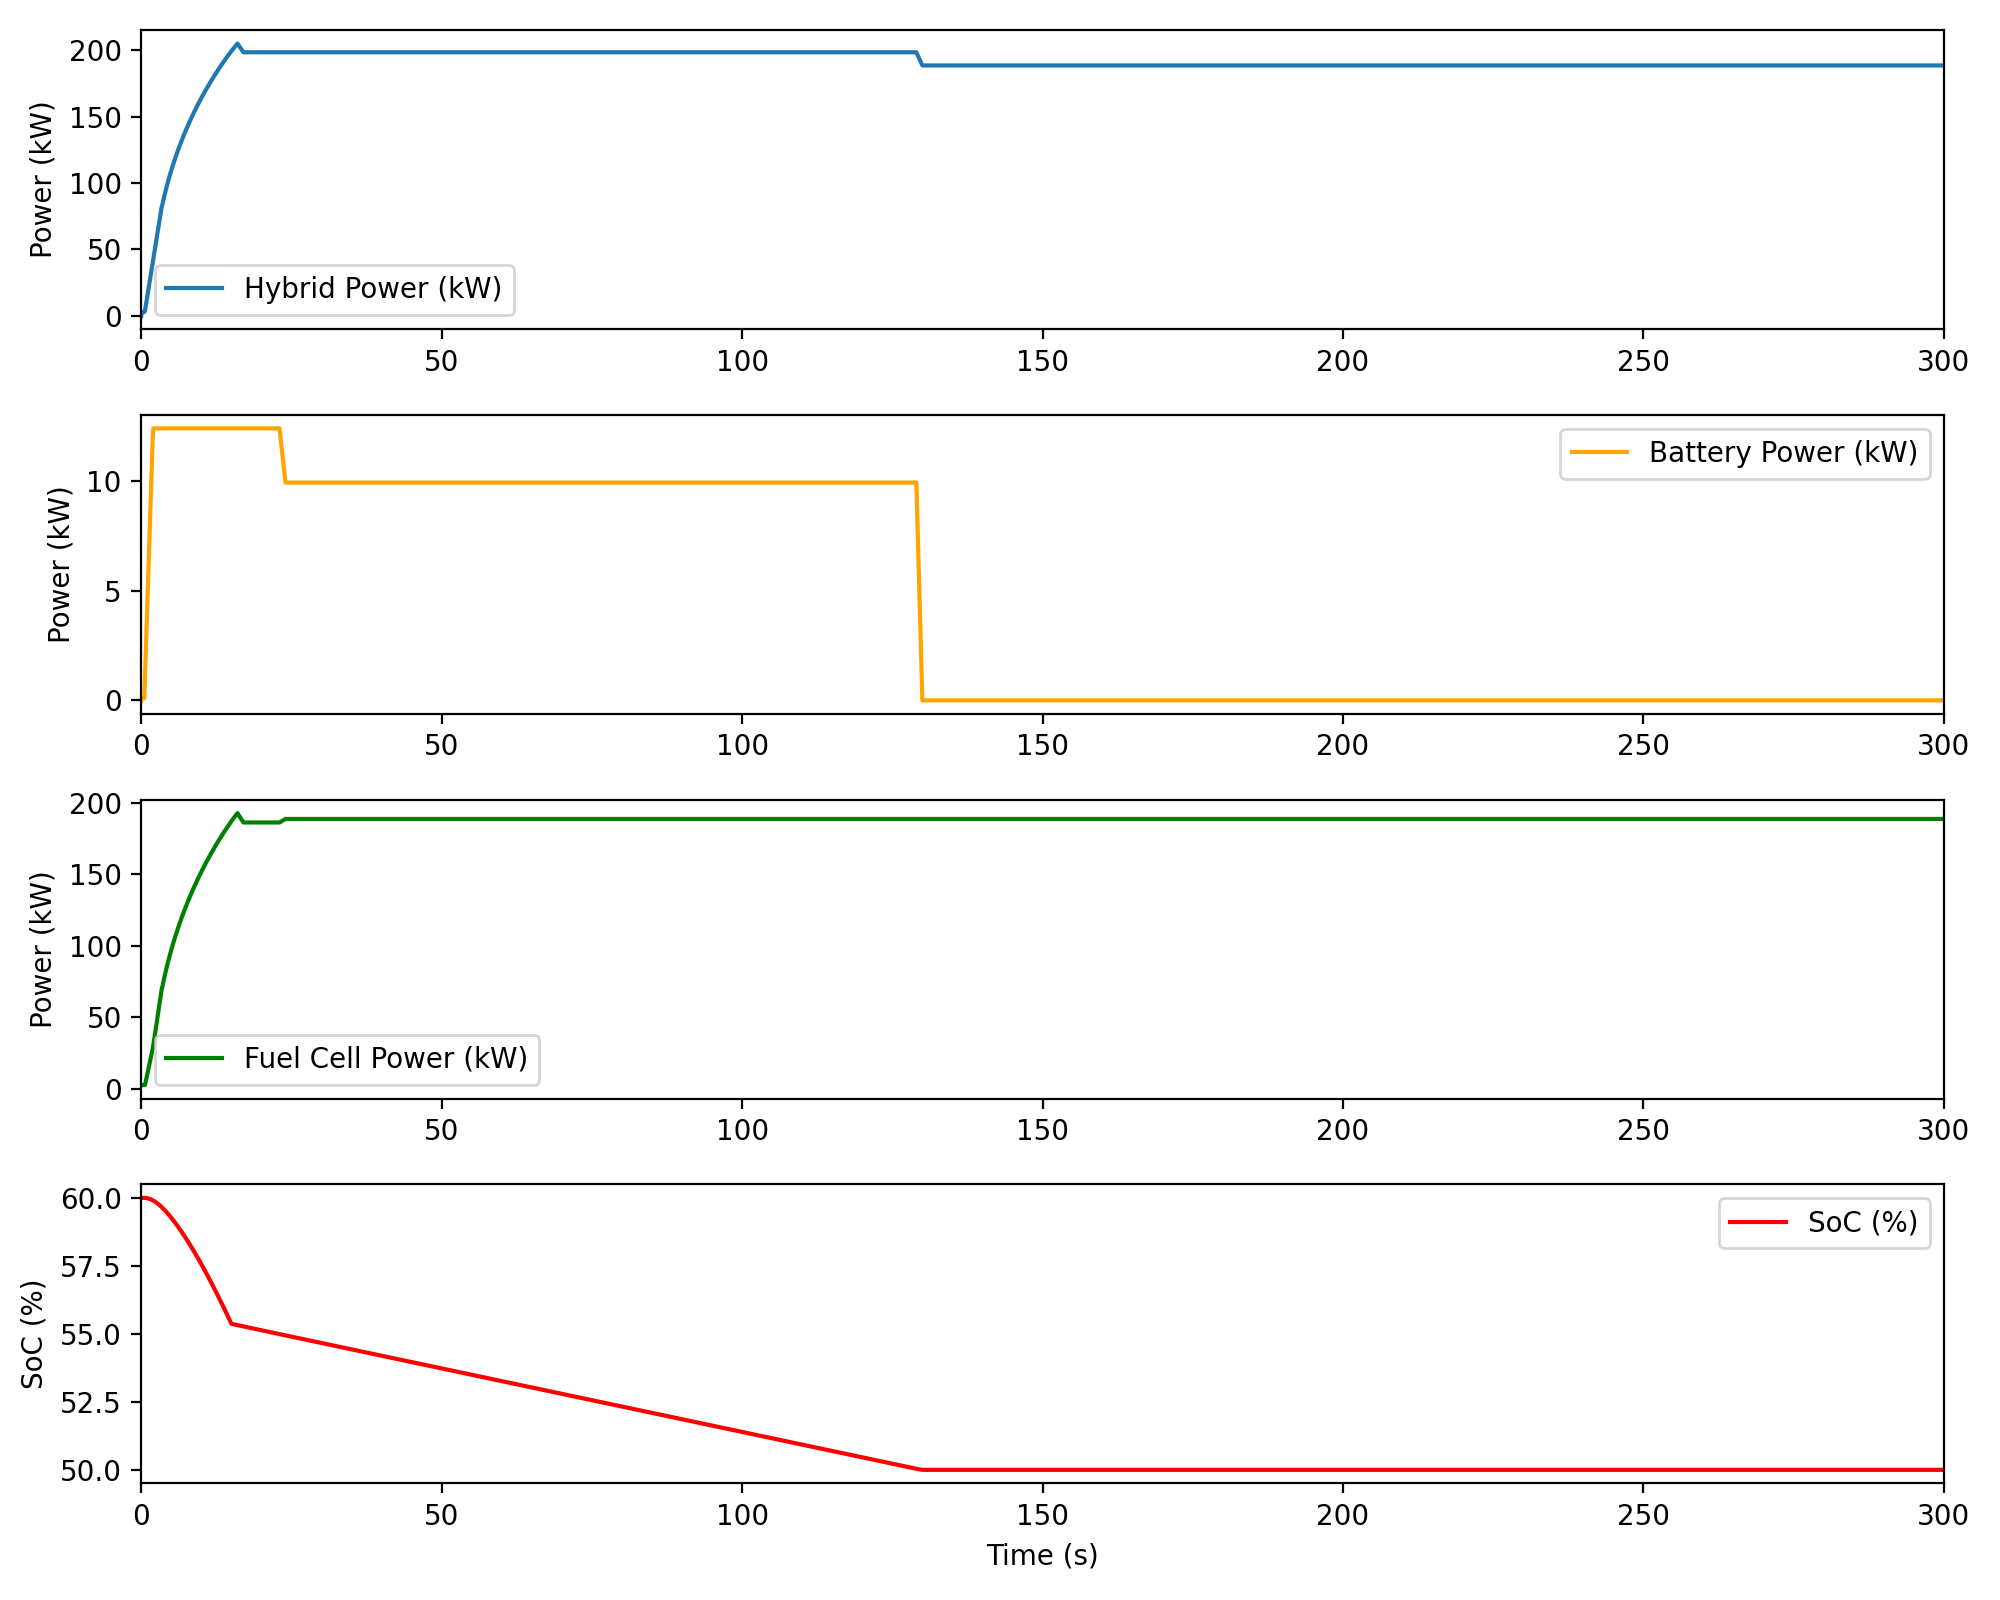
\includegraphics[width=0.95\linewidth]{E:/07. Master_Degree_ITC+UGA/02. ENES3_SGB_UGA/02. New Technology/PEMFC/Question_C_130_V2.png}
	\caption{\small {Hybrid working in Power transfer in Vehicle 130kmh}}
	\label{14}
\end{figure}

\begin{itemize}
	\item \textbf{Hybrid Power (kW) - Blue Curve (Top Plot):}
	\begin{itemize}
		\item The hybrid power increases sharply from 0 to about \textbf{17.45 kW} within the first few seconds.
		\item After this peak, the power stabilizes around \textbf{10.917 kW} and remains constant for the rest of the 300-second interval.
	\end{itemize}
	
	\item \textbf{Battery Power (kW) - Orange Curve (Second Plot):}
	\begin{itemize}
		\item The battery power rises rapidly to a maximum value of \textbf{5.24 kW} at the beginning and then drops slightly, stabilizing around \textbf{3.27 kW}.
		\item The battery maintains this output throughout the time period shown.
	\end{itemize}
	
	\item \textbf{Fuel Cell Power (kW) - Green Curve (Third Plot):}
	\begin{itemize}
		\item The fuel cell power ramps up initially to about \textbf{12.22 kW}.
		\item After reaching this maximum value, the fuel cell output drops slightly and stabilizes at around \textbf{7.64 kW} for the remainder of the time.
	\end{itemize}
	
	\item \textbf{State of Charge (SoC \%) - Red Curve (Bottom Plot):}
	\begin{itemize}
		\item The SoC starts at \textbf{60.0\%} and decreases gradually over time.
		\item By the end of the 300-second period, the SoC has dropped to \textbf{58.5\%}.
	\end{itemize}
\end{itemize}






%% =======================================1 . =========================================
% Sections and Subsections
\section{\underline{Analysis of the fuel cell system with WLTC profile}}

We assume that the fuel cell system of the vehicle has the following characteristics, based on some specifications of the Mirai 2 and an experimental study of the Mirai 1:

\begin{itemize}
	\item Hydrogen storage: 5.6 kg stored at 700 bars
	\item Molar mass of dihydrogen: 2.016 g/mol
	\item Enthalpy of hydrogen combustion in oxygen:
	\begin{itemize}
		\item LHV: 242 kJ/mol
		\item HHV: 285 kJ/mol
	\end{itemize}
	\item The hydrogen loss (mainly in the purge) represents 2\% of the consumed hydrogen
	\item Air stoichiometry is 1.5
	\item Atmospheric pressure is 1 bar
	\item Oxygen molar fraction in ambient air is 21\%
\end{itemize}

\begin{itemize}
	\item Air compressor's efficiency is 60\% (comprising both compression efficiency and electric motor efficiency)
	\item The stack is composed of 330 cells of 273 cm\(^2\)

\end{itemize}

%% ======================================= a . =========================================

\subsection{Calculate and Plot as a function of the stack current: }
\subsubsection{The electrical power consumed by the air compressor}

To calculate of the compression power are proportional to the current:
\begin{equation}
	P_{comp}(t) = \frac{1}{\eta_{sys}(t)}q_{m_{air}(t)}c_pT_e(\tau^{\frac{\gamma-1}{\gamma}}-1)\label{eq2.1}
\end{equation}

Where we got :

\begin{itemize}
	\item Air mass Flow : 
		\begin{equation}
			q_{m_{air}}(t) = M_{air}F_{air}(t) = M_{air} \frac{v_{air}}{x_{O_2}}\frac{N_{cell}I(t)}{4\mathscr{F}} = M_{air} \frac{v_{air}}{x_{O_2}}\frac{P_{sys}(t)}{2v_{H_2}(t)\rho_{sys}\Delta H} 
			\label{eq2.2}
		\end{equation}
	\item Heat Capacity:
		\begin{equation}
			c_p =\frac{\gamma}{\gamma-1}\frac{R}{M} \label{eq2.3}
		\end{equation}
	\item Compression ratio:
		\begin{equation}
			\tau = \frac{\textit{p}_{out}}{\textit{p}_{in}} \label{eq2.4}
		\end{equation}
\end{itemize}

Get Equation (\ref{eq2.2}), Equation (\ref{eq2.3}), Equation (\ref{eq2.4}) Substitution into Equation (\ref{eq2.1})

\begin{equation}
	P_{comp}(t) = \frac{1}{\eta_{sys}(t)} \frac{v_{air}}{x_{O_2}}\frac{N_{cell}I(t)}{4\mathscr{F}} \frac{\gamma}{\gamma-1}RT_e(\tau^{\frac{\gamma-1}{\gamma}}-1)\label{eq2.5}
\end{equation}

\begin{figure}[h]
	\centering 
	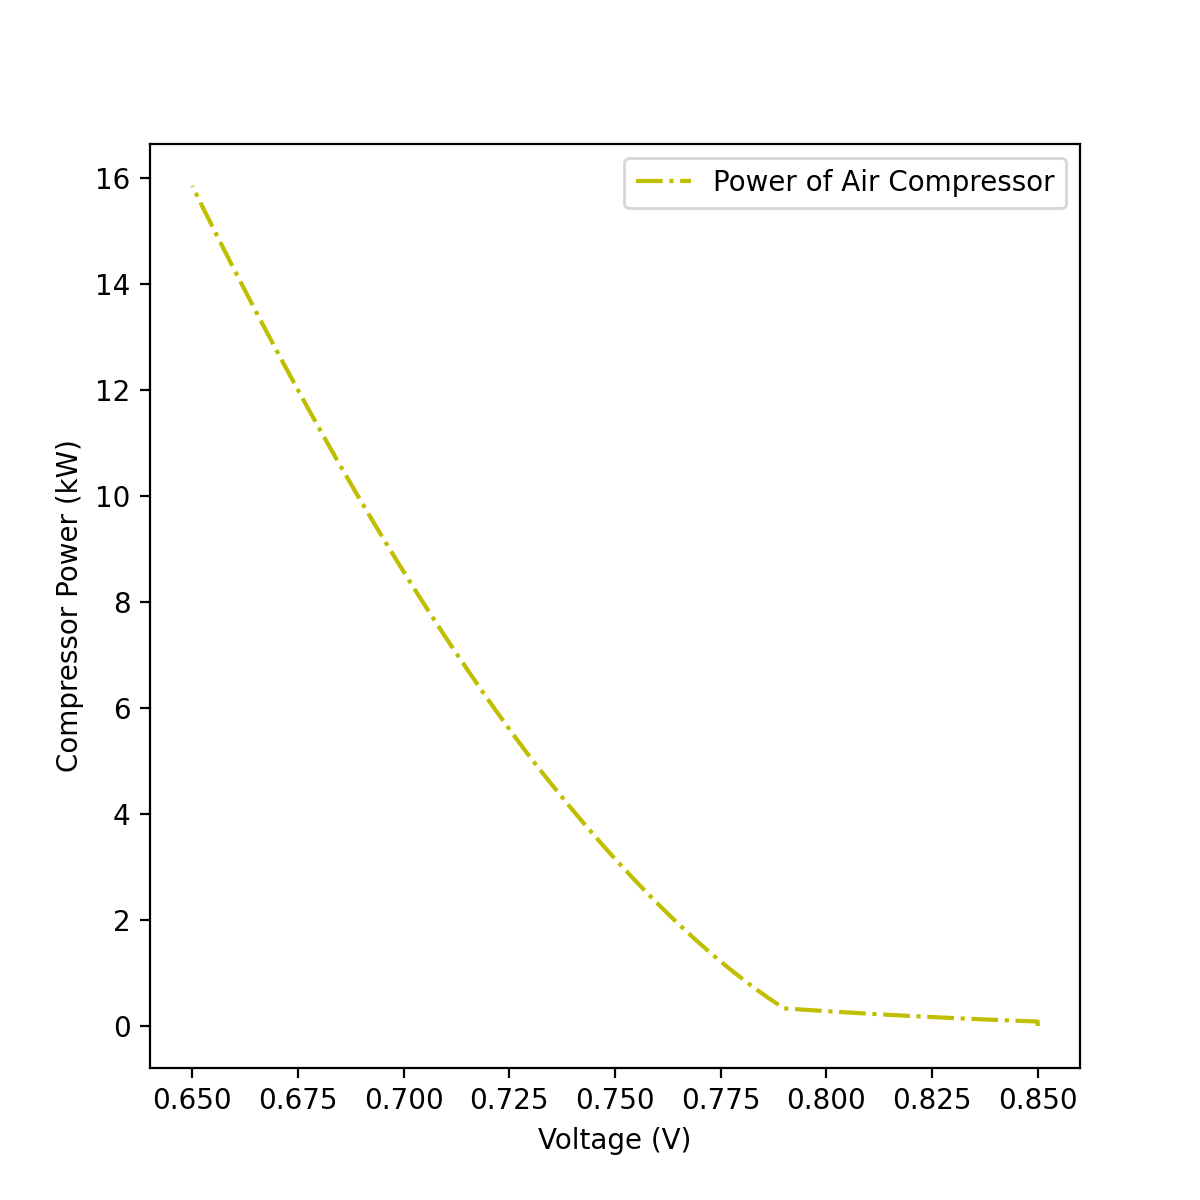
\includegraphics[width=0.9\linewidth]{E:/07. Master_Degree_ITC+UGA/02. ENES3_SGB_UGA/02. New Technology/PEMFC/Power_of_Air_compressor.png}
	\caption{\small {Power of Air Compressor}}
	\label{15}
\end{figure}

\begin{itemize}
	\item \textbf{Figure (\ref{15}) Top Plot: Power vs. Voltage (Yellow Dashed Curve)}
	\begin{itemize}
		\item The curve shows a downward trend as the voltage increases. It starts high on the left (at around 15 kW for a voltage near 0.65 V) and gradually declines, approaching zero as the voltage nears 0.85 V.
		\item The decrease is non-linear, with a steep drop at first and then leveling off as the voltage approaches higher values. This suggests that as voltage increases, the power output of the air compressor significantly reduces, particularly more rapidly at lower voltage values.
	\end{itemize}
	\item \textbf{Figure (\ref{15}) Bottom Plot: Power vs. Index (Green Solid Curve)}
	\begin{itemize}
		\item The curve exhibits a steady upward trend as the index increases. Starting close to 0 kW at a low index, it rises continuously, reaching around 15 kW at the highest index value.
		\item The increase appears almost linear, with a constant or slightly accelerating rate of power increase as the index progresses.
	\end{itemize}
\end{itemize}



%=======================================================================================================================


\subsubsection{The electrical power delivered by fuel cell system.}

To calculate the fuel cell that consumption in the system, we used: 
To find the hydrogen consumption, we will use: 
\begin{equation}
	P_{comp}(t) = U_{cell}\times i(t) \times N_{cell} \times A_{cell} \label{eq2.6}
\end{equation}

\begin{figure}[h]
	\centering 
	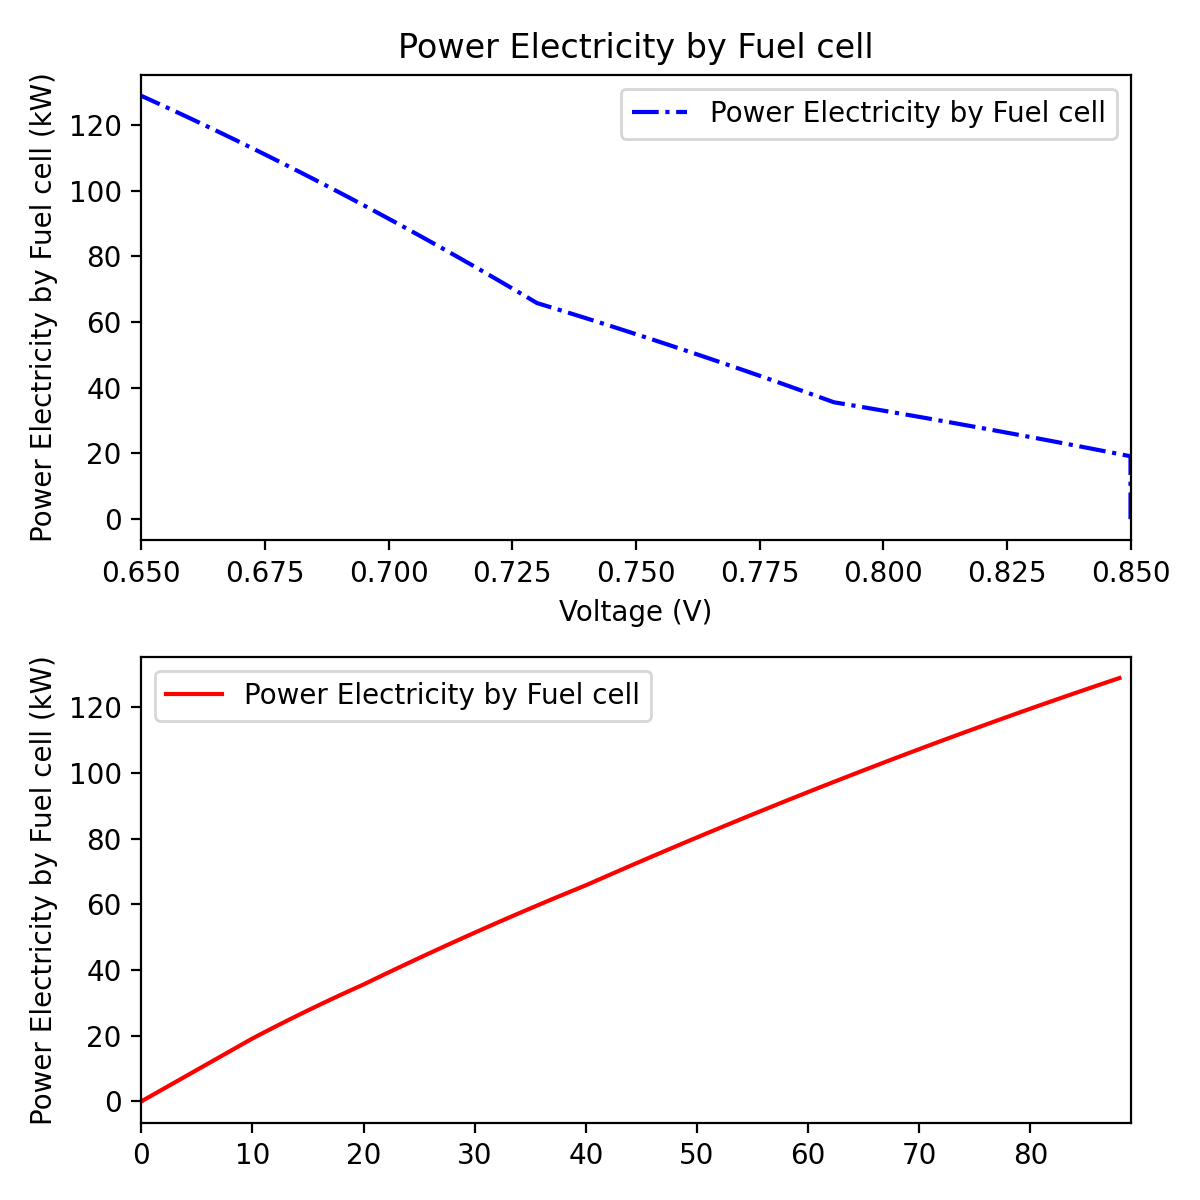
\includegraphics[width=0.9\linewidth]{E:/07. Master_Degree_ITC+UGA/02. ENES3_SGB_UGA/02. New Technology/PEMFC/Power_of_Fuel_Cell.png}
	\caption{\small {The electrical power delivered by fuel cell system}}
	\label{16}
\end{figure}
\begin{itemize}
	\item \textbf{Figure (\ref{16}) : Top Plot}
	\begin{itemize}
		\item The x-axis represents the \textbf{Voltage (V)} of the fuel cell, ranging from approximately 0.65V to 0.85V.
		\item The y-axis represents the \textbf{Power output} in watts, ranging from 0 to around 120 watts.
		\item The plot shows a \textbf{decreasing trend} as voltage increases, suggesting that power output drops as voltage rises. The line is \textbf{dash-dotted and blue}, indicating a measured or calculated trend of power with respect to voltage.
	\end{itemize}
	
	\item \textbf{Figure (\ref{16}) : Bottom Plot}
	\begin{itemize}
		\item The x-axis represents the \textbf{Index}, possibly indicating the step number or data point (e.g., time or sequence index), ranging from 0 to 90.
		\item The y-axis again represents \textbf{Power output} in watts, similar to the top plot.
		\item The plot shows a \textbf{steady increase} in power as the index increases, potentially reflecting the increase in power over time or due to increasing load. The line is \textbf{solid red}, representing a direct correlation between index and power output.
	\end{itemize}
\end{itemize}



%=======================================================================================================================


\subsubsection{The hydorgen consumption by the duel cell system. Fit the curve with a fifth degree polynomial.}
\begin{figure}[h]
	\centering 
	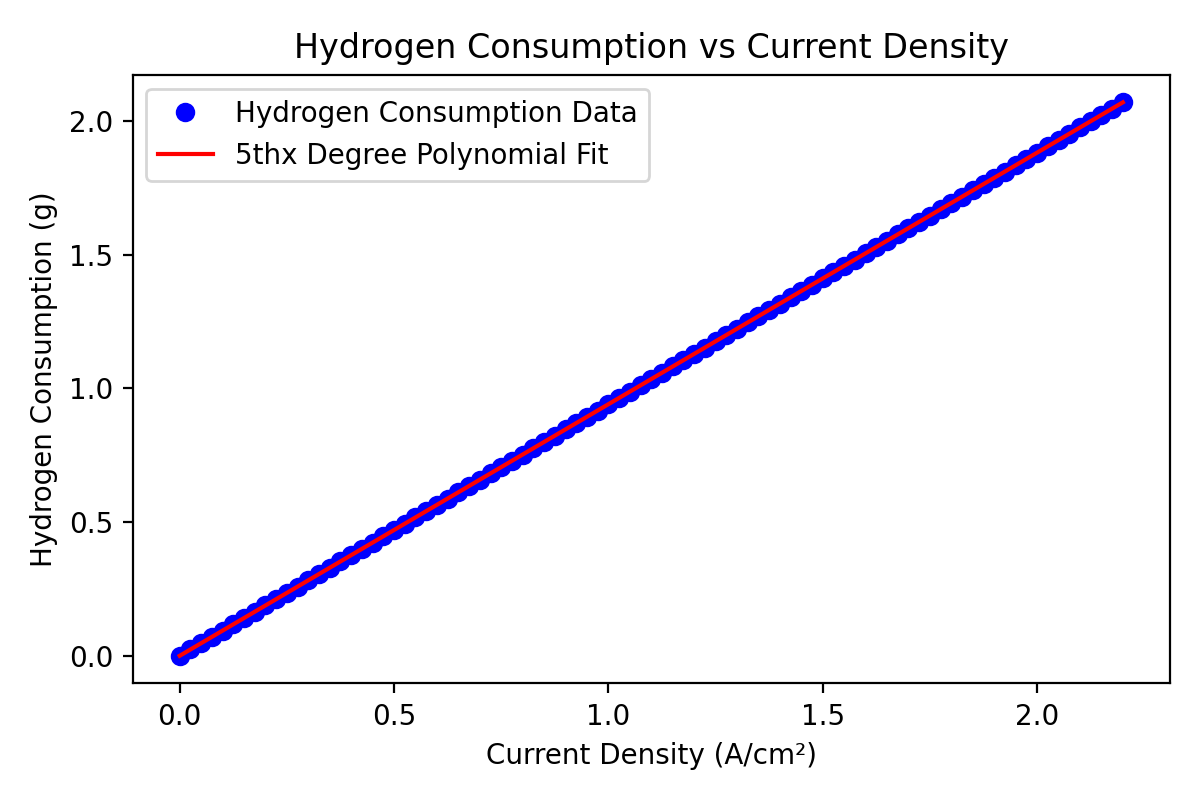
\includegraphics[width=0.8\linewidth]{E:/07. Master_Degree_ITC+UGA/02. ENES3_SGB_UGA/02. New Technology/PEMFC/Hydrogen Consumption vs Current Density in fit with fifth degree polynomial.png}
	\caption{\small {Hydrogen Consumption vs Current Density fit with fifth degree polynomial}}
	\label{17}
\end{figure}
\begin{itemize}
	\item Find the mole flow in the system : 
	\begin{equation}
		\dot{m}_{H_2}(t) = \frac{I(t)}{2\mathscr{F}}\times M_{H_2} \times N_{Cell} \times A_{cell} \label{eq2.7}
	\end{equation}

	\item Fifth-Degree Polynomial Equation
	\begin{equation}
		P(x) = a_5 x^5 + a_4 x^4 + a_3 x^3 + a_2 x^2 + a_1 x + a_0
	\end{equation}
	\item Hydrogen Consumption as a Function of Current Density:
	\begin{equation}
		P(i) = a_5 (i)^5 + a_4 (i)^4 + a_3 (i)^3 + a_2 (i)^2 + a_1 (i) + a_0
	\end{equation}
	\item $(a_0, a_1, a_2, a_3, a_4, a_5)$ : Coefficients of the polynomial, determined through the fitting process. These coefficients define the shape of the polynomial curve.
\end{itemize}
This graph displays in Figure (\ref{17}) the relationship between hydrogen consumption (in grams) and current density (in A/cm²)
\begin{itemize}
	\item \textbf{Data Points (Blue)}:
	\begin{itemize}
		\item The blue markers represent the experimental hydrogen consumption data at various current densities.
		\item A clear linear trend is observed, where hydrogen consumption increases as the current density increases.
	\end{itemize}
	
	\item \textbf{Polynomial Fit (Red Curve)}:
	\begin{itemize}
		\item The red line represents a 5th-degree polynomial fit to the data.
		\item Despite being a higher-order polynomial, the fit closely resembles a straight line, indicating a strong linear relationship between current density and hydrogen consumption.
	\end{itemize}
	
	\item \textbf{Linear Trend}:
	\begin{itemize}
		\item The plot shows that hydrogen consumption increases almost linearly with the current density in the range of 0 to 2 A/cm².
		\item This is expected in electrochemical systems, where fuel consumption is proportional to the current density.
	\end{itemize}
	
	\item \textbf{Accuracy of Fit}:
	\begin{itemize}
		\item The data points closely align with the polynomial fit, indicating a high degree of accuracy.
		\item The minimal deviation between the data and the fit suggests that a linear or near-linear model accurately describes the relationship.
	\end{itemize}
	
	\item \textbf{Practical Implication}:
	\begin{itemize}
		\item Increasing the current density results in a proportional increase in hydrogen consumption.
		\item This insight is important for fuel cell applications, where controlling current density helps manage fuel consumption.
	\end{itemize}
	
\end{itemize}

The graph effectively communicates that hydrogen consumption increases linearly with the current density over the given range.

%================================================2. b =======================================================================



\subsection{Considering the WLTC drive cycle, calculate and plot the instant hydrogen consumption in kg/s
as a function of time. Give the total amount of hydrogen consumed for one complete cycle. 
Calculate the average hydrogen consumption of the vehicle in kgH2/100 km. Deduce the vehicle 
operating range, and the average energetic efficiency.
}

To Calculate the value in this question, we will use servals equation :

\begin{itemize}
	\item To calculate the mass flow rate of hydrogen, we obtained :
	\begin{equation}
		\dot{m}_{H_2}(t) = \frac{I_{cell}(t)\times N_{cell}\times M_{H_2}}{2\mathscr{F}}
	\end{equation}
	\item To determine the Current of the cell, we used
	\begin{equation}
		I_{cell}(t) = \frac{\text{Power demand} (t)}{U_{cell}(t)}
	\end{equation}
	\item To obtained the Cell voltage, we use one of optimization method to fine the optimal voltage of the each cell depend on speed, time and power demand of the vehicle. We will Minimize Scalar Optimization to do it.
\begin{itemize}
	\item Let \( f(x) \) be a scalar function defined as:
	\begin{equation}
		f: \mathbb{R} \to \mathbb{R}
	\end{equation}
	
	\item The goal is to find \( x^* \) such that:
	\begin{equation}
		x^* = \arg \min_{x \in [a, b]} f(x)
	\end{equation}
	
	\item We may define constraints in optional bounds for \( x \):
	\begin{equation}
		a \leq x \leq b
	\end{equation}
	
	\item The optimization seeks to minimize the function:
	\begin{equation}
		\min_{x \in [a, b]} f(x)
	\end{equation}
	
	\item Several methods can be used in the \texttt{minimize\_scalar} function:
	\begin{itemize}		
		\item \textbf{Brent's Method}: A robust method that combines the bisection method, secant method, and inverse quadratic interpolation.
		\item \textbf{Golden Section Search}: A technique that systematically narrows the interval containing the minimum point.
		\item \textbf{Bounded Methods}: Enforces the constraints \( a \) and \( b \) while searching for the minimum.
	\end{itemize}
	
	\item If the function \( f \) is differentiable, the first derivative condition is applied:
	\begin{equation}
		f'(x^*) = 0
	\end{equation}
	
	\item To confirm that \( x^* \) is a local minimum, we use the second derivative condition:
	\begin{equation}
		f''(x^*) > 0
	\end{equation}
	
	\item The optimization algorithm will typically terminate when:
	\begin{itemize}
		\item The change in the objective function value is less than a specified tolerance level, \( \epsilon \):
		\begin{equation}
			|f(x_{k+1}) - f(x_k)| < \epsilon
		\end{equation}
		
		\item The change in \( x \) is less than a specified tolerance level, \( \delta \):
		\begin{equation}
			|x_{k+1} - x_k| < \delta
		\end{equation}
	\end{itemize}
\end{itemize}
\item To find the total hydorgen consumed, we can use :

	\begin{equation}
		\text{Total Hydrogen Consumption} = \int_{0}^{T}\dot{m}_{H_2}(t)dt
	\end{equation}

\item To detemine System Efficiency, we do :

\begin{equation}
	E_{\text{from H2}} = \frac{m_{\text{hydro}}[t] \cdot LHV_{\text{hydrogen}}}{M_{\text{olar mass H2}}} \quad \text{if } m_{\text{hydro}}[t] > 0
\end{equation}

\begin{equation}
	\eta[t] = 
	\begin{cases} 
		\frac{P_{\text{fuel cell}}}{E_{\text{from H2}}} & \text{if } E_{\text{from H2}} > 0 \\
		0 & \text{if } E_{\text{from H2}} \leq 0 
	\end{cases}
\end{equation}
\item To calculate the range operation of the vehicle:
	\begin{equation}
		d_{\text{traveled}} = v_s[1:] \cdot \Delta t
	\end{equation}
	
	\begin{equation}
		D_{\text{total}} = \frac{\sum d_{\text{traveled}}}{1000}
	\end{equation}
	
	\begin{equation}
		\text{Consumption of Hydrogen Average} = 
		\begin{cases} 
			\frac{{\text{Consumption of Hydrogen total}} \cdot 100}{D_{\text{total}}} & \text{if } D_{\text{total}} > 0 \\
			0 & \text{if } D_{\text{total}} \leq 0 
		\end{cases}
	\end{equation}
	
\begin{equation}
	R_{\text{operation}} = 
	\begin{cases} 
		\frac{\text{Capacity tank}}{\text{Consumption of Hydrogen Average}}} / 100} & \text{if }\text{Consumption of Hydrogen Average} > 0 \\
		0 & \text{if } \text{Consumption of Hydrogen Average} \leq 0 
	\end{cases}
\end{equation}


\end{itemize}

\begin{figure}[h]
	\centering 
	\includegraphics[width=1\linewidth]{E:/07. Master_Degree_ITC+UGA/02. ENES3_SGB_UGA/02. New Technology/PEMFC/Hydrogen_Mass_and_Efficiency.png}
	\caption{\small {Mass Flow rate of the Hydrogen and Efficiency of the System}}
	\label{18}
\end{figure}
From Figure (\ref{18}), the plot presents two graphs that examine hydrogen mass consumption and system efficiency over time, each shedding light on operational performance.

\begin{itemize}
	\item The first graph shows hydrogen mass consumption in kilograms per second across a duration of \textbf{0 to 1800} seconds. It displays considerable fluctuations, with distinct spikes occurring at various points. This variability indicates that the system undergoes changing operational demands, potentially driven by factors such as load variations or environmental influences.The total hydrogen consumed is \textbf{0.204508 kg}, indicating the total usage during the observed timeframe and the average hydrogen consumption is approximately \textbf{0.879134 kg(H$_2$)/100 km}, serving as a useful reference for assessing efficiency relative to distance traveled. 
	
	\item The second graph focuses on system efficiency, represented as a percentage, within the same time frame. Efficiency varies between \textbf{30\%} and \textbf{70\%}, suggesting that the system doesn't operate at a steady level. With an average system efficiency of around \textbf{61.74\%}, the data reflects a moderate level of performance throughout the observed period. Additionally, the operation range is reported to be \textbf{643.82 km}, which may relate to the effective distance achieved based on hydrogen usage and efficiency. The fluctuations in efficiency highlight potential areas where operational improvements could be made.
	\item The relationship between hydrogen consumption and system efficiency is crucial to this analysis. The changes in hydrogen consumption can directly affect efficiency, with higher consumption periods possibly linked to lower efficiency levels. Identifying these patterns and understanding their underlying causes can offer valuable insights for optimizing system performance. Analyzing the factors that lead to low efficiency during certain periods will be vital for refining operational strategies. Collecting further data on load conditions and external factors during these fluctuations could deepen the analysis and help improve overall performance in hydrogen-dependent applications.
\end{itemize}




%%============================================2. c =======================================================




\subsection{Sensitivity analysis - observe the effect of the following variations on the results obtained in the previous question}
\begin{itemize}
	\item Varation of C:
	\begin{itemize}
		\item C = 0,25
		\item C = 0.40
	\end{itemize}

	\item Varation of Cr:
	\begin{itemize}
		\item Cr = 0.01
		\item Cr = 0.014
	\end{itemize}

	\item Variation of bateery charging Power:
	\begin{itemize}
		\item Battery Charging = 5C
		\item Battery Charging = 20C
	\end{itemize}

	\item Variation of the battery capacity :
	
	\begin{itemize}
		\item Battery Capacity  = 620 Wh or 0.62 kWh
		\item Battery Capaity = 1860 Wh or 1.86 kWh
	\end{itemize}
\end{itemize}


In this question , we will devided the input parameter into two main part: 

\begin{itemize}
	\item First : $C = 0.25$ , $Cr = 0.01$, Battery Charging = $5C$,$20C$ and Battery Capacity = $0.62 kWh$
	\item Second : $C = 0.40$ , $Cr = 0.014$, Battery Charging = $5C$,$20C$ and Battery Capacity = $1.86 kWh$
\end{itemize}


\subsubsection{First : $C = 0.25$ , $Cr = 0.01$, Battery Charging = $5C$,$20C$ and Battery Capacity = $0.62 kWh$}

\begin{figure}[h]
	\centering 
	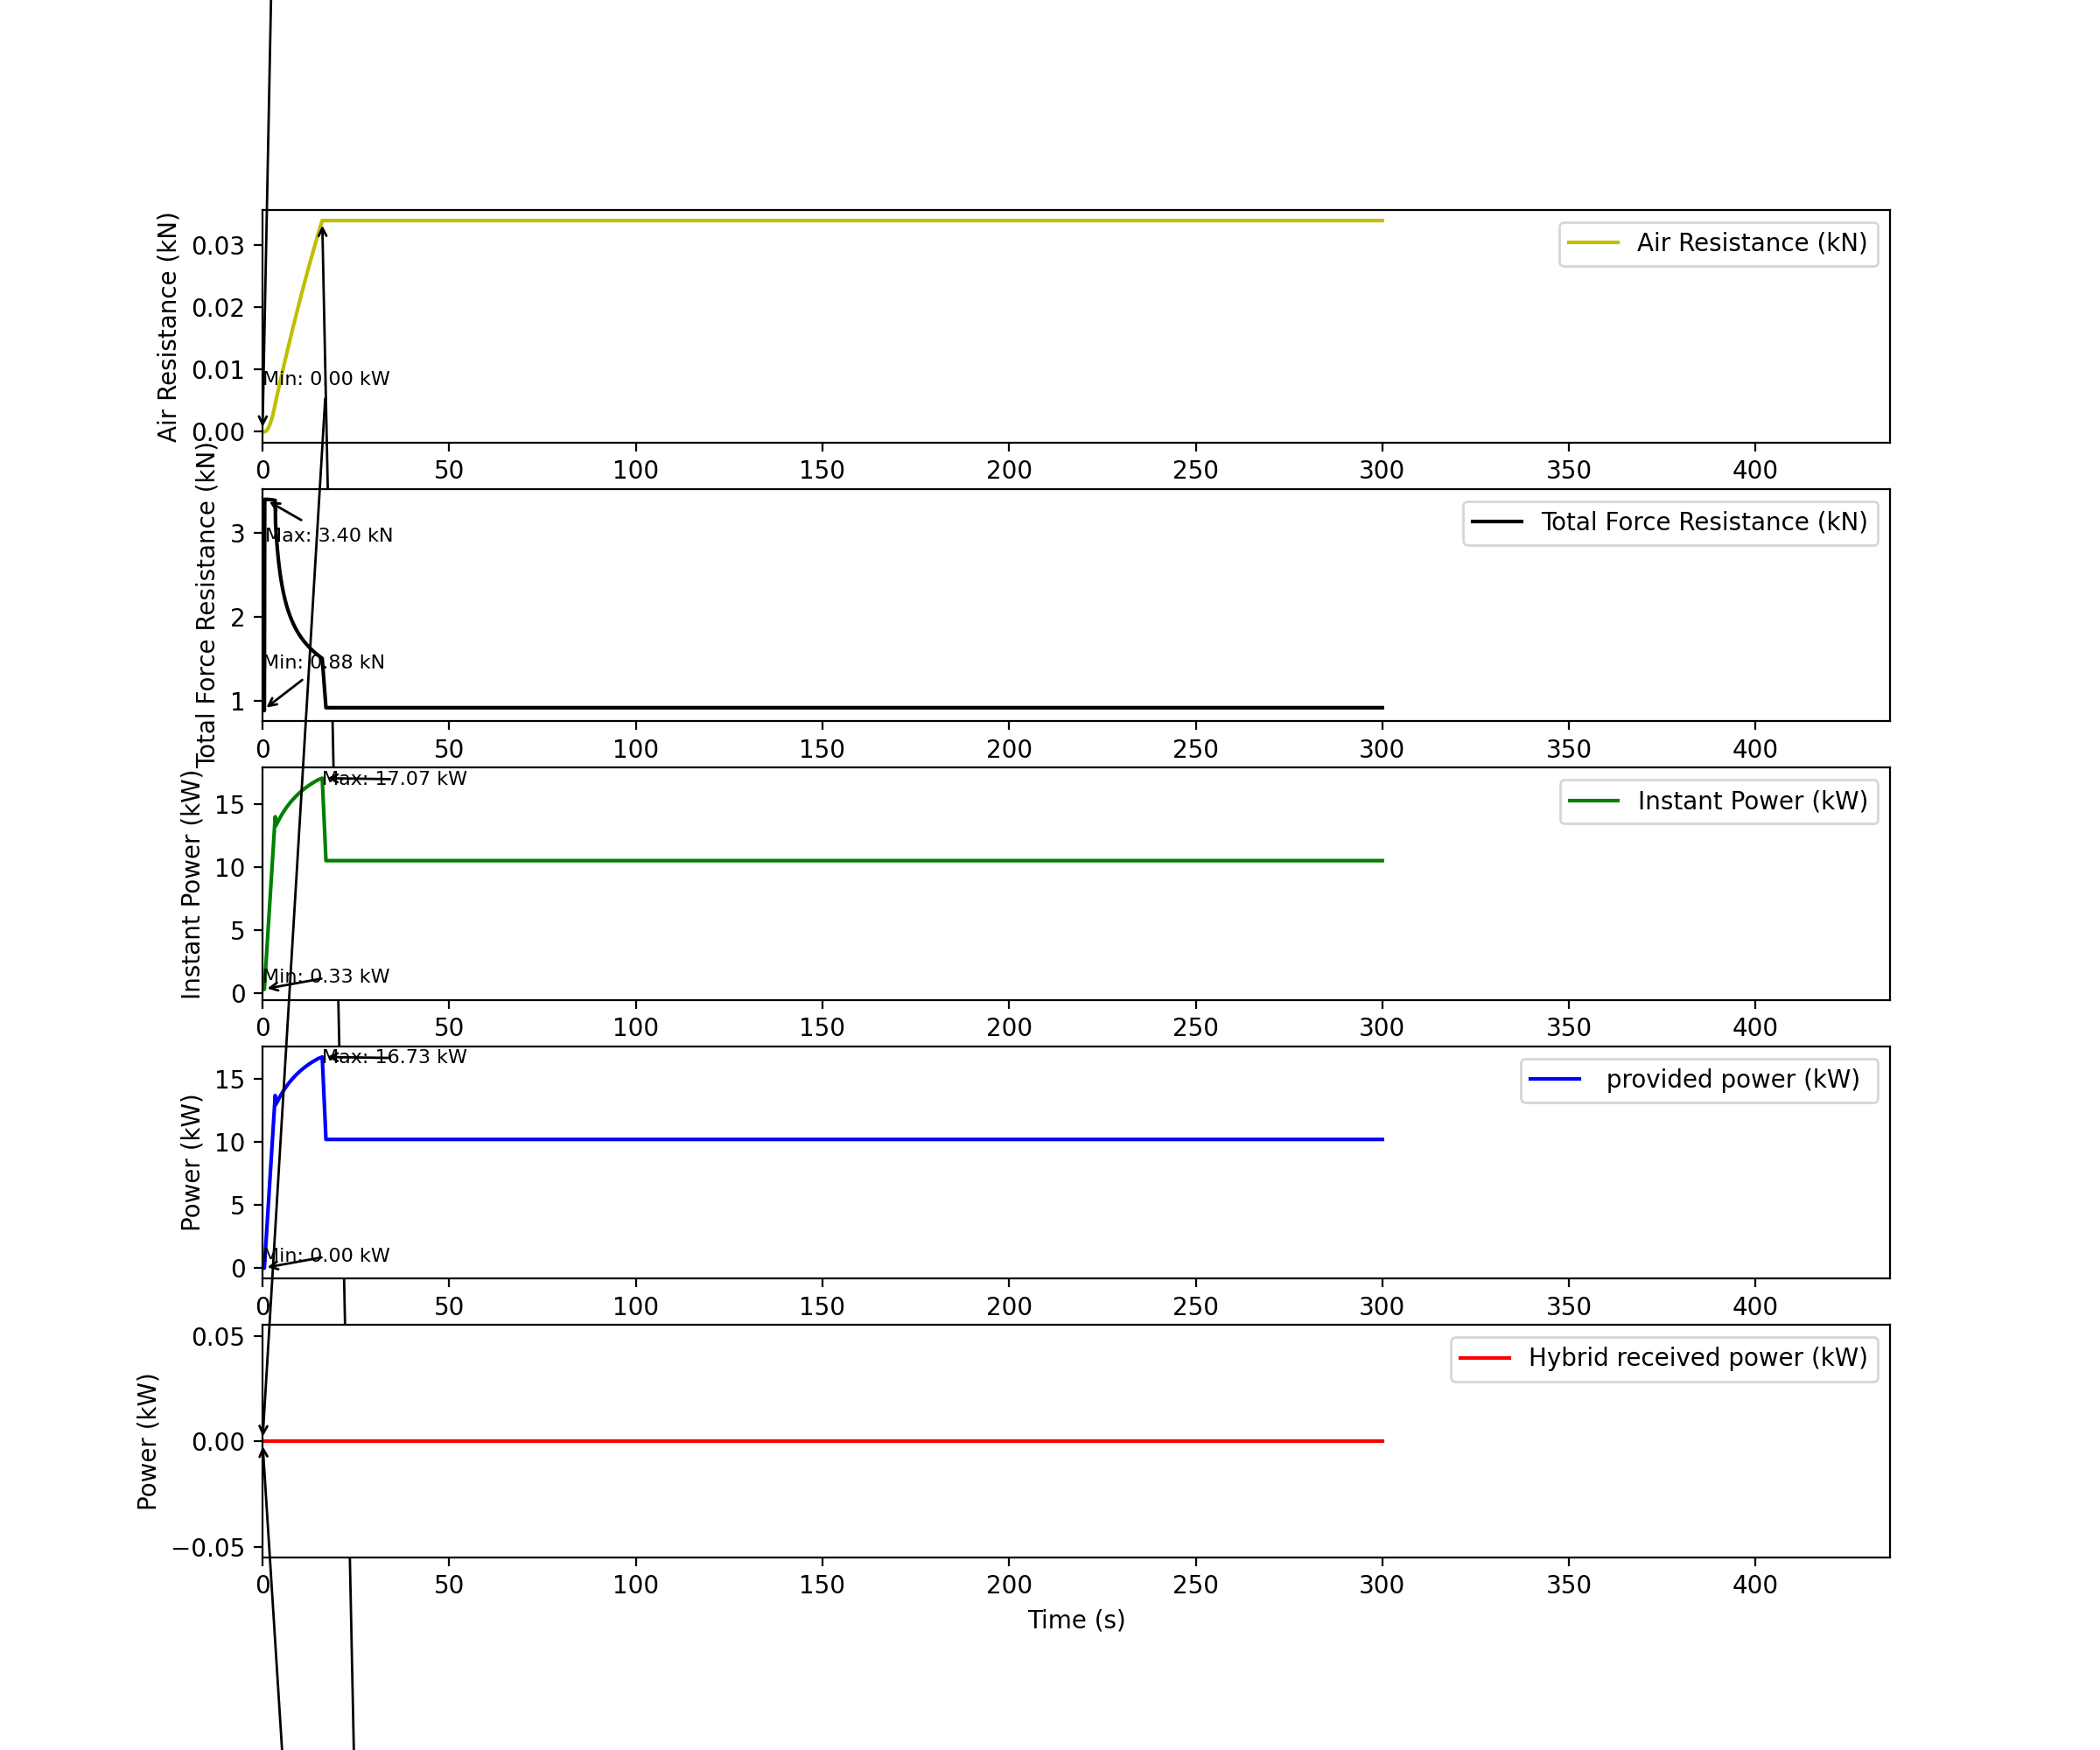
\includegraphics[width=1\linewidth]{E:/07. Master_Degree_ITC+UGA/02. ENES3_SGB_UGA/02. New Technology/PEMFC/C1/Question_A.png}
	\caption{\small {Curve of Air Resistance, Total Force, Instant Power, Hybrid Provided and Received Power}}
	\label{19}
\end{figure}
As, we used to do at the previous Section(1) we assumed that:
\begin{itemize}
	\item By looking between the Figure (\ref{4})a with Figure (\ref{19}) yellow curve, we can see that air resistance likely decrease while the maximum air resistance force at Figure (\ref{4})a was around \textbf{500 N} but in Figure (\ref{19}) is around \textbf{450 N}.
	\item For the total resistance force of vehicle from previous question in Figure (\ref{4})b slightly the same value of maximum and minimum of the value that we calculate in this question shown on the Figure (\ref{19}) black curve. 
	\item As the result of the Total force resistance of previous question between this question calculation likely the same. We can assumed that the Instant power, Hybrid power received and provided of pervious question shown by Figure (\ref{7}) with this question calculation shown by Figure (\ref{19}) (Green, Blue and Red curve) are slightly the same characteristic as pervious one.
	\begin{itemize}
		\item The maximum, minimun of Instant Power of this question around \textbf{57.37 kW} and \textbf{34.60 kW} . So, we can said that the maximum of hybrid system will provided to the system is around \textbf{57.37 kW} and received \textbf{34.60 kW}.
		\item The maximum, minimun of Instant Power of this question around \textbf{58.488 kW} and \textbf{34.365 kW}
	\end{itemize}
\end{itemize}

\begin{figure}[h]
	\centering 
	\includegraphics[width=1\linewidth]{E:/07. Master_Degree_ITC+UGA/02. ENES3_SGB_UGA/02. New Technology/PEMFC/C1/Question_C.png}
	\caption{\small {Hydrid System, Battery Manangement, Fuel Cell Power and State of Charge of the Vehicle}}
	\label{20}
\end{figure}
\begin{itemize}
	\item \textbf{Hybrid Power (kW):}
	\begin{itemize}
		\item {Figure (\ref{20}):} The range goes up to maximum about \textbf{57.37 kW}, with frequent fluctuations between 0 and 60 kW, and a few drops below 0 kW to the minimum of \textbf{24.80 kW}. Moreover, this figure is more dynamic behavior where power transitions between positive and negative more frequently, showing a more active power management system that involves energy recovery (negative power).
		\item {Figure (\ref{8}):} The hybrid power fluctuates significantly between 0 and \textbf{58.82 kW} and the minimum is just \textbf{7.44 kW} below 0. There are high peaks with fewer negative values, implying a system that mostly generates or draws power in positive ranges.
	\end{itemize}
	
	\item \textbf{Battery Power (kW):}
	\begin{itemize}
		\item {Figure (\ref{20}):} Similarly, the maximum range of charging is \textbf{24.8 kW} and and discharging range is \textbf{12.4 kW}. While in {Figure (\ref{8}):} the maximum chargine is juat \textbf{7.44 kW} and maximum range of discharge almost \textbf{12.40 kW}. 
		\item For the Figure (\ref{8}) lightly broader range with more focus on discharging power.
		On the other hand, For the Figure (\ref{20}) is clearer fluctuations between charging and discharging, emphasizing a balance in battery management between supplying and recovering energy.
	\end{itemize}
	
	\item \textbf{Fuel Cell Power (kW):}
	\begin{itemize}
		\item {Figure (\ref{20}):} The data shows similar behavior, with sharp spikes and a max value of \textbf{44.97 kW}. The power stays within the same range.
		\item {Figure (\ref{8}):} Tuel cell power remains mostly positive, fluctuating between 0 and max value of \textbf{46.42 kW}. The curve is characterized by sharp peaks followed by rapid declines.
	\end{itemize}
	
	\item \textbf{State of Charge (SoC):}
	\begin{itemize}
		\item {Figure (\ref{8}):} he SoC starts around \textbf{60\%} and drops steadily over time, reaching a minimum of \textbf{56.28\%}. The curve shows a consistent decline, with a larger total drop in SoC.
		\item {Figure (\ref{20}):} The SoC also starts at \textbf{60\%} but drops more slowly, reaching a minimum of \textbf{53.60\%}. The decline is less pronounced compared to the Figure (\ref{8}) and SoC has drop deeply than Figure (\ref{8}) because of the capacity of battery is 0.62 kWh compare with Figure (\ref{8}) is 1.24kWh
	\end{itemize}

	
\end{itemize}

\begin{figure}[h]
	\centering 
	\includegraphics[width=1\linewidth]{E:/07. Master_Degree_ITC+UGA/02. ENES3_SGB_UGA/02. New Technology/PEMFC/C1/Hydrogen_Mass_and_Efficiency.png}
	\caption{\small {Hydrid System, Battery Manangement, Fuel Cell Power and State of Charge of the Vehicle}}
	\label{21}
\end{figure}

At the Previous question that shown in the Figure (\ref{18}) and our calculation at the moment in the Figure(\ref{21}):

\begin{itemize}
	\item For the Total Hydrogen Consumed at the Figure (\ref{18}) is around \textbf{0.2045 kg} with \textbf{0.8791 kg(H$_2$)/100km} while the Total Hydrogen Consumed at this question is around \textbf{0.189 kg} with \textbf{0.8148 kg(H$_2$)/100km} and it is coming from the Power of the Hybrid system based on time decreased.
	
	\item Average System Efficiency is \textbf{61.74\%} with \textbf{643.82km} Operation Range at the previous question. In contract, at moment the Average System Efficiency is slightly dropped to \textbf{61.06\%} but the operation range is approximately increasing to \textbf{687.28 km} because of the Power demand decreasing becuase of the total force and other main reasons.
	
\end{itemize} 

\subsubsection{Second : $C = 0.40$ , $Cr = 0.014$, Battery Charging = $5C$,$20C$ and Battery Capacity = $1.86 kWh$}














\end{document} 